\documentclass[oneside,a4paper,12pt]{article}
\usepackage[english,brazilian]{babel}
\usepackage{multicol}
\usepackage{textcomp}
\usepackage[alf]{abntex2cite}
\usepackage[utf8]{inputenc}
\usepackage[T1]{fontenc}
\usepackage{amsmath,amssymb,exscale}
\usepackage[top=20mm, bottom=20mm, left=20mm, right=20mm]{geometry}%margens cima, baixo, esquerda direita
\usepackage{framed}
\usepackage{booktabs} %Pacote para deixar tabelas mais bonitas.
\usepackage{color} %Pacote de Cores
\usepackage{hyperref} %Pacotes para Hiperlinks
\usepackage{graphicx} %Pacote de imagens
\graphicspath{{./Figuras/}}%Direciona as imagens para uma pasta chamada "Figuras" (uso isso para organizar. Uma vez que todas as imagens vao ficar em uma pasta isolada)    
\definecolor{shadecolor}{rgb}{0.8,0.8,0.8}


%%%%%

\newtheorem{proposition}{Proposição}[section]
\newtheorem{theorem}{Teorema}[section]
\newtheorem{lemma}{Lema}[section]
\newtheorem{definition}{Definição}[section]
\newtheorem{conjecture}{Conjectura}[section]
\newtheorem{corollary}{Corolário}[section]
\newtheorem{proof}{Demonstração}

%%%%%

%FAZ EDICOES AQUI (somente no conteudo que esta entre entre as ultimas  chaves de cada linha!!!)
\newcommand{\universidade}{Universidade Tecnológica Federal do Paraná}
\newcommand{\centro}{Câmpus Cornélio Procópio}
\newcommand{\departamento}{Departamento Acadêmico de Matemática}
\newcommand{\curso}{Turma Especial}
\newcommand{\professores}{Matheus Pimenta}
\newcommand{\disciplina}{Geometria Analítica e Álgebra Linear - EC31G}
%\newcommand{\tema}{Lista 01}
%\newcommand{\turma}{MA31G}
%\newcommand{\data}{Março de 2019}%{\today}
%\newcommand{\tempodeaula}{30 minutos}
%\newcommand{\prerequisitos}{Matrizes, Transformações Lineares e Bases}
%ATE AQUI !!!	

\begin{document}

	\begin{center}
		
\includegraphics[width=\linewidth/8]{logo.jpg}%LOGOTIPO DA INSTITUICAO
	 	\vspace{2pt} 	
		
		\universidade
		\par
		\centro
		\par
		\departamento
		\par
	%	Curso de \curso
		\par
		\vspace{12pt}
		\LARGE \textbf{Notas de Aula}
		
	\end{center}
	
	\vspace{12pt}
	
	\begin{tabular}{ |l|p{12cm}| }
		
		\hline
		\multicolumn{2}{|c|}{\textbf{Dados de Identificação}} \\
		\hline
		Professor:         &    \professores           \\
		\hline
		Disciplina:        &    \disciplina          \\
		\hline
	%	Tema:              &    \tema                \\
	%	\hline
	%	Pré-requisito	:  &    \prerequisitos         \\
	%	\hline
	%	Aluno:             &                   \\
	%	\hline
	%	Data:              &    \data                \\
	%	\hline
	%	Duração da aula:   &    \tempodeaula         \\
	%	\hline
		
	\end{tabular}
	\vspace{6pt}
	
	
	\begin{snugshade}
		\section{Sistema de Coordenadas}
	\end{snugshade}

\subsection{Coordenadas de um Ponto no Plano}

Em 1619, o filósofo e matemático francês René Descartes (1596-1650) percebeu que a ideia de determinar posições utilizando retas, escolhidas como referência, poderia ser aplicado à matemática. Para isso usou retas numeradas.

Descartes resolveu este problema usando duas retas numeradas, perpendiculares, cortando-se na origem. Usualmente, uma dessas retas é horizontal, com a direção positiva para a direita. Esta reta será chamada eixo $x$ ou eixo das abscissas. A outra reta, vertical com a direção positiva para cima, é chamada eixo $y$, ou eixo das ordenadas. 

 cada ponto $P$ do plano fica associado um par de números $(x,y)$, que são as coordenadas deste ponto. O número $x$ é chamado abscissa desse ponto, e o número $y$ é a sua ordenada. O número $x$ mede a distância orientada do ponto P ao eixo $y$ , e o número $y$ mede a distância orientada do ponto $P$ ao eixo $x$.
	
Se $P$ tem coordenadas $x$ e $y$ escrevemos $P(x,y)$.

\vspace{190pt}
\begin{center}
	\textcolor{red}{FIGURA 01 - PLANO CARTESIANO}
\end{center}

Todo ponto $P$ determina um par ordenado de números reais e reciprocamente, todo par ordenado de números reais $(a,b)$ determina um único ponto do plano. Temos então uma correspondência biunívoca entre os pontos do plano e os pares ordenados de números reais. Uma correspondência desse tipo é chamada um {\it sistema de coordenadas no plano} ou {\it sistema de coordenadas cartesianas}.

O eixo das abscissas e o eixo das ordenadas, usualmente colocados na posição indicada na figura abaixo, dividem o plano em quatro regiões, denominadas quadrantes.

\vspace{180pt}
\begin{center}
	\textcolor{red}{FIGURA 02 - PLANO CARTESIANO COM QUADRANTES}
\end{center}
 
 O primeiro quadrante é o conjunto de todos os pontos $(x,y)$ do plano para os quais $x>0$ e $y>0$; o segundo quadrante é o conjunto de todos os pontos $(x,y)$ do plano para os quais $x<0$ e $y>0$; no terceiro temos $x<0$ e $y<0$ e, no quarto, $x>0$ e $y<0$.  
 
 Como a correspondência entre os pontos do plano e o conjunto de pares ordenados de números reais é biunívoca, em geral, nos referimos a um ponto P como o ponto $(1,2)$ ou o ponto $(x,y)$ quando, na realidade queremos nos referir ao ponto P cujas coordenadas são $(1,2)$ ou $(x,y)$.
 
 
\subsection{Coordenadas de um Ponto no Espaço} 
 
{\bf Sistema cartesiano ortogonal no espaço:} no espaço tridimensional adiciona-se um terceiro eixo, o eixo $z$ ou eixo das cotas. Os três eixos: ordenada, abscissa e cota, dividem o espaço em oito partes chamadas de octantes ou oitantes.
 
No espaço um ponto fica caracterizado por uma tripla, chamada de terna: $$P = (x,y,z)$$

\vspace{180pt}
\begin{center}
	\textcolor{red}{FIGURA 03 - ESPAÇO}
\end{center}


Dimensões maiores: para quatro ou mais dimensões os eixos adicionais não tem mais nomes, mas a propriedade deles serem ou não ortogonais para definirmos sistemas de coordenadas ortogonais ou não continua válida.

As seguintes observações são válidas:
\begin{itemize}
	\item a origem do sistema de eixos ortogonais é o ponto $O = (0,0,0)$;
	\item os eixos do sistema são os conjuntos: \\
	$$ eixo - OX = \{(x,0,0) ; x \in \mathbb{R} \}$$
	$$eixo - OY = \{(0,y,0) ; y \in \mathbb{R} \}$$
	$$eixo - OZ = \{(0,0,z) ; z \in \mathbb{R} \}$$
	\item os planos cartesianos são os conjuntos: \\
	$$\pi_{XY} = \{(x,y,0); x,y \in \mathbb{R} \}$$
	ou seja, $\pi_{XY} : z = 0$ \\
	$$\pi_{XZ} = \{(x,0,z); x,z \in \mathbb{R} \}$$
	ou seja, $\pi_{XZ} : y = 0$ \\	
	$$\pi_{YZ} = \{(0,y,z); y,z \in \mathbb{R} \}$$
	ou seja, $\pi_{YZ} : x = 0$ 	
\end{itemize}

Um sistema de coordenadas cartesianas no espaço $\varepsilon$ permite descrever todos os subconjuntos do espaço por meio das coordenadas de seus pontos.


\begin{snugshade}
	\section{Matrizes}
\end{snugshade}

Aparecem na resolução de problemas, pois ordenam e simplificam dados, fornecendo métodos de resolução.

\textbf{Exemplo: }Uma indústria de roupas necessita das seguintes matéria prima: golas, malha, ribana, botão e linha ou estampa, bordado e corte.

O primeiro padrão de produção é o seguinte:
\begin{table}[h]
	\centering
\begin{tabular}{|c|c|c|c|c|}
	\hline
		&	Camisa		&	Polo	&	Camiseta& 	Regata\\
	\hline
Linha	&	1			&	1		&	1		&	1	\\	
	\hline
Golas	&	1			&	1		&	0		&	0	\\
	\hline
Malha	&	3			&	2		&	2		&	1	\\
	\hline
Ribana	&	0			&	0		&	1		&	1	\\
	\hline
Botão	&	10			&	2		&	0		&	0	\\
	\hline			
\end{tabular}
\end{table}

Um segundo padrão de produção é o seguinte
\begin{table}[h]
	\centering
	\begin{tabular}{|c|c|c|c|c|}
		\hline
				&	Camisa		&	Polo	&	Camiseta& 	Regata\\
		\hline
		Estampa	&	0			&	1		&	2		&	1	\\	
		\hline
		Bordado	&	1			&	1		&	1		&	0	\\
		\hline
		Corte	&	5			&	5		&	4		&	3	\\
		\hline
	\end{tabular}
\end{table}

Reescrevendo em forma matricial:

O padrão $1$ é o seguinte:
	$\left[
	\begin{array}{cccc}		
	1			&	1		&	1		&	1	\\	
	1			&	1		&	0		&	0	\\
	3			&	2		&	2		&	1	\\
	0			&	0		&	1		&	1	\\
	10			&	2		&	0		&	0	\\		
	\end{array}
	\right]
	$
	
O padrão $2$ é o seguinte:
	$\left[
	\begin{array}{cccc}
	0			&	1		&	2		&	1	\\	
	1			&	1		&	1		&	0	\\
	5			&	5		&	4		&	3	\\
	\end{array}
	\right]$


\begin{definition}[Matriz]
	Uma matriz é um conjunto de elementos dispostos em $m$ linhas e $n$ colunas:
	
	$$
	\left[
	\begin{array}{cccc}
	a_{11}	&	a_{12}	&	\dots	&	a_{1n}	\\
	a_{21}	&	a_{22}	&	\dots	&	a_{2n}	\\
	a_{31}	&	a_{32}	&	\dots	&	a_{3n}	\\
	\vdots	&	\vdots	&	\dots	&	\vdots	\\
	a_{m1}	&	a_{m2}	&	\dots	&	a_{mn}	\\
	\end{array}
	\right]
	$$
\end{definition}

\subsection{Tipos de Matrizes}

Considere uma matriz com $m$ linhas e $n$ colunas, denotada por $A_{m \times n}$.

\subsubsection{Matriz Quadrada}
É quando $m=n$ e então dizemos que $A$ é de ordem $m$.

\textbf{Exemplo: }

\begin{multicols}{3}
	$
	\left[
	\begin{array}{ccc}
	3	&	6	&	32	\\
	5	&	8	&	0	\\
	6	&	12	&	1	\\
	\end{array}
	\right]
	$
	
	$
	\left[
	\begin{array}{cc}
	1	&	0	\\
	0	&	1	\\
	\end{array}
	\right]
	$
	
	$
	\left[
	\begin{array}{c}
	9	\\
	\end{array}
	\right]
	$
\end{multicols}

\subsubsection{Matriz Nula}

Todos os elementos são nulos, ou seja, $a_{ij} = 0$.

\textbf{Exemplo: }

\begin{multicols}{3}
	$
	\left[
	\begin{array}{ccc}
	0	&	0	&	0	\\
	0	&	0	&	0	\\
	\end{array}
	\right]
	$
	
	$
	\left[
	\begin{array}{cc}
	0	&	0	\\
	0	&	0	\\
	\end{array}
	\right]
	$
	
	$
	\left[
	\begin{array}{c}
	0	\\
	\end{array}
	\right]
	$
\end{multicols}

\subsubsection{Matriz Coluna}

Ocorre quando $n=1$ e $m$ é qualquer.

\textbf{Exemplo: }

\begin{multicols}{2}
	$
	\left[
	\begin{array}{c}
	0	\\
	2	\\
	6	\\
	9	\\
	1	\\
	\end{array}
	\right]
	$
	
	$
	\left[
	\begin{array}{c}
	24	\\
	43	\\
	\end{array}
	\right]
	$
	
\end{multicols}

\subsubsection{Matriz Linha}

Ocorre quando $m=1$ e $n$ é qualquer.

\textbf{Exemplo: }

\begin{multicols}{2}
	$
	\left[
	\begin{array}{ccccc}
	0	&	12	&	4	&	32	&	1
	\end{array}
	\right]
	$
	
	$
	\left[
	\begin{array}{ccc}
	24	&	1	&	9
	\end{array}
	\right]
	$
	
\end{multicols}

\subsubsection{Matriz Diagonal}

É no caso quando:
\begin{itemize}
	\item $m=n$;
	\item $a_{ij}=0$ para todo $i \neq j$
\end{itemize}

\textbf{Exemplo: }

\begin{multicols}{2}
	$
	\left[
	\begin{array}{ccc}
	3	&	0	&	0	\\
	0	&	32	&	0	\\
	0	&	0	&	1	\\
	\end{array}
	\right]
	$
	
	$
	\left[
	\begin{array}{cc}
	3	&	0	\\
	0	&	7	\\
	\end{array}
	\right]
	$
	
\end{multicols}

\subsubsection{Matriz Identidade}

Ocorre no caso:
\begin{itemize}
	\item $m=n$;
	\item $a_{ij}=0$ para todo $i \neq j$;
	\item $a_{ii}=1$
\end{itemize}

\textbf{Exemplo: }

\begin{multicols}{2}
	$
	\left[
	\begin{array}{ccc}
	1	&	0	&	0	\\
	0	&	1	&	0	\\
	0	&	0	&	1	\\
	\end{array}
	\right]
	$
	
	$
	\left[
	\begin{array}{cc}
	1	&	0	\\
	0	&	1	\\
	\end{array}
	\right]
	$
	
\end{multicols}

\subsubsection{Matriz Triangular Superior}

É a seguinte:
\begin{itemize}
	\item $m=n$;
	\item $a_{ij}=0$ para todo $i > j$;
\end{itemize}

\begin{multicols}{2}
	$
	\left[
	\begin{array}{cccc}
	2	&	2	&	0	&	-4	\\
	0	&	-1	&	4	&	5	\\
	0	&	0	&	23	&	-10	\\
	0	&	0	&	0	&	3
	\end{array}
	\right]
	$
	
	$
	\left[
	\begin{array}{ccc}
	2	&	1	&	3	\\
	0	&	7	&	2	\\
	0	&	0	&	3
	\end{array}
	\right]
	$
	
\end{multicols}


\subsubsection{Matriz Triangular Inferior}

É a seguinte:
\begin{itemize}
	\item $m=n$;
	\item $a_{ij}=0$ para todo $i < j$;
\end{itemize}

\begin{multicols}{2}
	$
	\left[
	\begin{array}{cccc}
	7	&	0	&	0	&	0	\\
	21	&	1	&	0	&	0	\\
	4	&	3	&	3	&	0	\\
	67	&	-9	&	3	&	2
	\end{array}
	\right]
	$
	
	$
	\left[
	\begin{array}{ccc}
	21	&	0	&	0	\\
	1	&	-5	&	0	\\
	5	&	2	&	-6
	\end{array}
	\right]
	$
	
\end{multicols}


\subsubsection{Matriz Simétrica}

É a seguinte:
\begin{itemize}
	\item $m=n$;
	\item $a_{ij}=a_{ji}$
\end{itemize}

$$
\left[
\begin{array}{cccc}
a	&	b	&	c	&	d	\\
b	&	e	&	f	&	g	\\
c	&	f	&	h	&	i	\\
d	&	g	&	i	&	k
\end{array}
\right]
$$


\subsection{Operações com Matrizes}

\subsubsection{Adição de Matrizes}
Duas matrizes de mesma ordem $A_{m \times n}$ e $B_{m \times n}$, podem ser somadas, operando os elementos correspondentes:

$$A + B = [a_{ij} + b_{ij}]_{m \times n}$$

\textbf{Exemplo: }


	$
	\left[
	\begin{array}{ccc}
	1	&	2	&	4	\\
	-3	&	2	&	7	\\
	3	&	10	&	9	\\
	\end{array}
	\right]
	$
	$+$
	$
	\left[
	\begin{array}{ccc}
	2	&	0	&	12	\\
	2	&	-5	&	-3	\\
	6	&	2	&	-6
	\end{array}
	\right]
	$
	$=$
	$
	\left[
	\begin{array}{ccc}
	3	&	2	&	16	\\
	-1	&	-3	&	4	\\
	9	&	12	&	3
	\end{array}
	\right]
	$	
	

\textbf{Propriedades da Adição}

Sejam $A$,$B$ e $C$ matrizes de ordem $m \times n$.
\begin{enumerate}
	\item Comutativa \\ $A+B=B+A$ 
	\item Associativa \\$(A+B)+C=A+(B+C)$ 
	\item Elemento Neutro \\ $A+0=A$, onde $0$ é a matriz nula de ordem $m \times n$ \\ \textbf{Obs. } $A+(-A)=0$ onde $-A$ é a matriz oposta
\end{enumerate}

\textbf{Demonstrações - Exercícios}

\subsubsection{Multiplicação por Escalar}

Sejam $A_{m \times n}$ e $k \in \mathbb{R}$, definimos $k \cdot A = [k \cdot a_{ij}]_{m \times n}$

\textbf{Exemplo: }

$2$ $\cdot$
$
\left[
\begin{array}{ccc}
3	&	2	&	16	\\
-1	&	-3	&	4	\\
9	&	12	&	3
\end{array}
\right]
$	
 $=$
$
\left[
\begin{array}{ccc}
6	&	4	&	32	\\
-2	&	-6	&	8	\\
18	&	24	&	6
\end{array}
\right]
$

\textbf{Propriedades: } Dadas as matrizes $A$ e $B$ de ordem $m \times n$ e números $k, k_1$ e $k_2 \in \mathbb{R}$, são válidas:
\begin{enumerate}
	\item Distributiva \\ $k(A+B)=kA+kB$
	\item Distributiva \\ $(k_1 + k_2)A = k_{1}A+k_{2}A$
	\item $0 \cdot A = 0_{m \times n}$, onde $0 \in \mathbb{R}$
	\item Associativa \\ $k_1(k_{2}A) = (k_{1}k_{2})A$
\end{enumerate}

\textbf{Demonstrações - Exercícios}

\subsubsection{Multiplicação de Matrizes}

Sejam $A_{m \times n}$ e $B_{n \times p}$, definimos $A \cdot B = C_{m \times p}$ onde:
\begin{itemize}
	\item [] $A = [a_{ij}]_{m \times n}$
	\item [] $B = [b_{rs}]_{n \times p}$
	\item [] $C = [c_{uv}]_{m \times p}$
\end{itemize}
e $c_{uv} = \sum_{k=1}^{n}a_{vk}\cdot b_{kv} + \dots + a_{vn} \cdot b_{nv}$

\textbf{Exemplo: }
$
\left[
\begin{array}{cc}
2	&	1	\\
4	&	2	\\
5	&	3
\end{array}
\right]
$
$\cdot$
$
\left[
\begin{array}{cc}
1	&	-1	\\
0	&	4	
\end{array}
\right]
$
$=$
$
\left[
\begin{array}{cc}
	2	&	2	\\
	4	&	4	\\
	5	&	7
\end{array}
\right]
$

\textbf{Propriedades: }
Sejam $A$, $B$ e $C$ matrizes com as ordens compatíveis para a realização da multiplicação entre sí, são válidas:
\begin{enumerate}
	\item $AI = IA = A$, onde $I$ é a matriz identidade
	\item $A(B+C) = AB + AC$
	\item $(A+B)C = AC + BC$
	\item $(AB)C = A(BC)$
	\item $0\cdot A = A \cdot 0 = 0$
	\item $(AB)^t = B^t \cdot A^t$
\end{enumerate}
\textbf{Obs. }Em geral não é valida a comutativa: $AB \neq BA$.

\textbf{Demonstrações - Exercícios}

\subsubsection{Transposição}

Dada $A_{m \times n}$, podemos obter $A_{n \times m}^{t}$ cujas linhas de $A^t$ são as colunas de $A$. $A^t$ é chamada de matriz transposta.

\textbf{Exemplo: }

$A =$
$
\left[
\begin{array}{cc}
2	&	2	\\
4	&	4	\\
5	&	7
\end{array}
\right]
$
e
$A^t=$
$
\left[
\begin{array}{ccc}
2	&	4	&	5	\\
2	&	4	&	7	\\
\end{array}
\right]
$

\textbf{Propriedades: }
\begin{enumerate}
	\item A matriz $A$ é simétrica $\Leftrightarrow A = A^t$ \\
	$
	\left[
	\begin{array}{cccc}
	a	&	b	&	c	&	d	\\
	b	&	e	&	f	&	g	\\
	c	&	f	&	h	&	i	\\
	d	&	g	&	i	&	k
	\end{array}
	\right]
	$
	$=$
		$
	\left[
	\begin{array}{cccc}
	a	&	b	&	c	&	d	\\
	b	&	e	&	f	&	g	\\
	c	&	f	&	h	&	i	\\
	d	&	g	&	i	&	k
	\end{array}
	\right]
	$
	\item $(A^t)^t = A$
\end{enumerate}


\subsection{Determinante de uma Matriz}

É uma função matricial que associa cada matriz quadrada a um escalar. É de grande importância para definir se uma matriz é inversível ou não.

Inicialmente tomemos algumas definições preliminares.

\begin{definition}
	Seja $I_n$ o conjunto dos $n$ primeiros números naturais. Exemplo: $I_3=\{1,2,3\}$, uma permutação em $I_n$ é uma função bijetora $P:I_n \rightarrow I_n$. 
	
	Por $I_n$ ser finito, $P$ é bijetora se, e somente se, $P$ é injetora.
\end{definition}

\textbf{Exemplo: } Seja $I_3$, apresente as permutações de $I_3$.

Para $I_3$ temos $3!$ funções bijetoras definidas sobre $I_3$, que são:
\begin{multicols}{3}
$
P(1)=
\left( 
\begin{array}{ccc}
1	&	2	&	3	\\
1	&	2	&	3
\end{array}
\right)
$

$
P(2)=
\left( 
\begin{array}{ccc}
1	&	2	&	3	\\
1	&	3	&	2
\end{array}
\right)
$

$
P(3)=
\left( 
\begin{array}{ccc}
1	&	2	&	3	\\
3	&	2	&	1
\end{array}
\right)
$

$
P(4)=
\left( 
\begin{array}{ccc}
1	&	2	&	3	\\
2	&	1	&	3
\end{array}
\right)
$

$
P(5)=
\left( 
\begin{array}{ccc}
1	&	2	&	3	\\
3	&	1	&	2
\end{array}
\right)
$

$
P(6)=
\left( 
\begin{array}{ccc}
1	&	2	&	3	\\
2	&	3	&	1
\end{array}
\right)
$

\end{multicols}

No caso das linhas serem iguais, denomina-se como {\it permutação identidade}, como no caso de $P(1)$.

\begin{definition}[Permutações par e ímpar]
	Uma permutação é definida como par, quando o número de trocas para transformá-la na permutação identidade é um número par, analogamente, uma permutação será definida como ímpar, quando o número de trocas para transformá-la na permutação identidade é um número ímpar. Só pode-se efetuar troca de dois números por vez de lugar.
\end{definition}

\textbf{Exemplo: } A permutação $P(2)$ necessita apenas de uma troca para obter a permutação identidade, sendo assim, uma permutação ímpar.

Já a permutação $P(5)$ necessita de duas trocas, sendo uma permutação par.

\begin{definition}[Sinal da Permutação]
	O sinal de uma permutação é definido por $sinal(P)=+1$ se $P$ é par e $sinal(P)=-1$ se $P$ é ímpar.
\end{definition}

\textbf{Exemplo: } As permutações $P(1), P(5)$ e $P(6)$ são permutações pares, enquanto as permutação $P(2),P(3)$ e $P(4)$ são ímpares.

\begin{definition}[Determinante de uma Matriz]
	Seja $\mathbb{M}(\mathbb{K})$ o espaço vetorial de todas as matrizes quadradas de ordem $n$ tendo escalares em um corpo $\mathbb{K}$ e $P_n$ o conjunto de todas as permutações de elementos de $I_n={1,2,3,\dots,n}$.
	
	Define-se a função determinante: $\det:\mathbb{M}(\mathbb{K}) \rightarrow \mathbb{K}$ que associa cada matriz $A \in\mathbb{M}(\mathbb{K})$, o escalar denotado por $\det(A)$, definido por:	
	
	$$\det(A) = \sum_{P \in P_{n}} sinal(P) a_{1P(1)}a_{2P(2)}a_{3P(3)}\dots a_{nP(n)}$$
	
	A soma acima deve ser realizada para $todas$ as permutações $P$ que pertencem ao conjunto $P_n$.
\end{definition}

\textbf{Exemplo: } Considere uma matriz $3 \times 3$:
$$
\left[
\begin{array}{ccc}
a_{11}	&	a_{12}		&	a_{13}	\\
a_{21}	&	a_{22}		&	a_{23}	\\
a_{31}	&	a_{32}		&	a_{33}	\\
\end{array}
\right]
$$

Utilizando as permutações de $I_3$
\begin{multicols}{3}
	$
	P(1)=
	\left( 
	\begin{array}{ccc}
	1	&	2	&	3	\\
	1	&	2	&	3
	\end{array}
	\right)
	$
	
	$
	P(2)=
	\left( 
	\begin{array}{ccc}
	1	&	2	&	3	\\
	1	&	3	&	2
	\end{array}
	\right)
	$
	
	$
	P(3)=
	\left( 
	\begin{array}{ccc}
	1	&	2	&	3	\\
	3	&	2	&	1
	\end{array}
	\right)
	$
	
	$
	P(4)=
	\left( 
	\begin{array}{ccc}
	1	&	2	&	3	\\
	2	&	1	&	3
	\end{array}
	\right)
	$
	
	$
	P(5)=
	\left( 
	\begin{array}{ccc}
	1	&	2	&	3	\\
	3	&	1	&	2
	\end{array}
	\right)
	$
	
	$
	P(6)=
	\left( 
	\begin{array}{ccc}
	1	&	2	&	3	\\
	2	&	3	&	1
	\end{array}
	\right)
	$
	
\end{multicols}

Temos que:

\begin{table}[h]
	\centering
	\begin{tabular}{|c|c|c|}
		\hline
	$P_1(1)=1$		&	$P_1(2)=2$		&	$P_1(3)=3$	\\
		\hline
	$P_2(1)=1$		&	$P_2(2)=3$		&	$P_2(3)=2$	\\
	\hline	
	$P_3(1)=3$		&	$P_3(2)=2$		&	$P_3(3)=1$	\\
\hline
	$P_4(1)=2$		&	$P_4(2)=1$		&	$P_4(3)=3$	\\
\hline
	$P_5(1)=3$		&	$P_5(2)=1$		&	$P_5(3)=2$	\\
\hline
	$P_6(1)=2$		&	$P_6(2)=3$		&	$P_6(3)=1$	\\
\hline
	$sinal(P_1)=1$	&	$sinal(P_2)=-1$	&	$sinal(P_3)=-1$	\\
\hline	
	$sinal(P_4)=-1$	&	$sinal(P_5)=1$	&	$sinal(P_6)=1$	\\
\hline		
	\end{tabular}
\end{table}


Assim:
\begin{eqnarray*}
	\det(A) &=& \sum_{P \in P_{3}} sinal(P) a_{1P(1)}a_{2P(2)}a_{3P(3)}	\\
	&=& sinal(P_1) a_{1P1(1)}a_{2P1(2)}a_{3P1(3)}	\\
	&+& sinal(P_2) a_{1P2(1)}a_{2P2(2)}a_{3P2(3)}	\\
	&+& sinal(P_3) a_{1P3(1)}a_{2P3(2)}a_{3P3(3)}	\\
	&+& sinal(P_4) a_{1P4(1)}a_{2P4(2)}a_{3P4(3)}	\\
	&+& sinal(P_5) a_{1P5(1)}a_{2P5(2)}a_{3P5(3)}	\\
	&+& sinal(P_6) a_{1P6(1)}a_{2P6(2)}a_{3P6(3)}	\\
	&=& a_{11}a_{22}a_{33}+a_{13}a_{21}a_{32}+a_{12}a_{23}a_{31}-a_{11}a_{23}a_{32}-a_{13}a_{22}a_{31}-a_{12}a_{21}a_{33}
\end{eqnarray*}

Que é a forma conhecida.

\textbf{Propriedades: }Segue algumas propriedades de determinantes.

\begin{enumerate}
	\item Se todos os elementos de uma linha (ou coluna) de $A$ são nulos, então $\det(A)=0$. \\ Já que em cada termo do cálculo do determinante há um dos elementos da linha (ou colunas) nula.
	\item $\det(A)=\det(A^t)$ \\ Se $A=[a_{ij}]$ e $A^t=[a_{ji}]$ as propriedades válidas para as linhas, são válidas para as colunas.
	\item Se multiplicarmos uma linha de $A$ por uma constante, $\det(A)$ é multiplicado pela constante. \\ Seja a matriz original e $B$ a matriz obtida de $A$ multiplicando uma linha de $A$ por $k$. No $\det(B)$, em cada termo, aparece um elemento dessa linha, podemos colocar $k$ em evidência e obter $\det(B) = k \cdot \det(A)$.
	\item Ao permutar duas linhas da matriz, o determinante troca de sinal, pois alteramos a paridade do número de inversões dos índices.
	\item Se $A$ tem duas linhas (ou colunas) iguais, seu determinante é nulo, isto é $\det(A)=0$. \\ Se trocarmos as linhas iguais o determinante é o mesmo, já que pela propriedade $4$, o determinante só pode ser $0$.
	\item $\det(A \cdot B) - \det(A) \cdot \det(B)$
\end{enumerate}
	

\subsubsection{Desenvolvimento de Laplace}

O objetivo do Desenvolvimento de Laplace é realizar o cálculo de determinantes de matrizes de ordem $n$, no caso $\det (A)_{n \times m}$.

Anteriormente já mostramos que se $A$ possui ordem $3$, então seu determinante é:

$$
\left[
\begin{array}{ccc}
a_{11}	&	a_{12}		&	a_{13}	\\
a_{21}	&	a_{22}		&	a_{23}	\\
a_{31}	&	a_{32}		&	a_{33}	\\
\end{array}
\right]
=
a_{11}a_{22}a_{33}+a_{13}a_{21}a_{32}+a_{12}a_{23}a_{31}-a_{11}a_{23}a_{32}-a_{13}a_{22}a_{31}-a_{12}a_{21}a_{33}
$$

Pode-se escrever como:

$$
a_{11}(a_{22}a_{33}-a_{23}a_{32})-a_{12}(a_{21}a_{33}-a_{23}a_{31})+a_{13}(a_{21}a_{32}-a_{22}a_{31})
$$

Ou ainda:
\begin{center}
$a_{11}
\left|
\begin{array}{cc}
a_{22}	&	a_{23}	\\
a_{32}	&	a_{33}	\\
\end{array}
\right|
-
a_{12}
\left|
\begin{array}{cc}
a_{21}	&	a_{23}	\\
a_{31}	&	a_{33}	\\
\end{array}
\right|
+
a_{13}
\left|
\begin{array}{cc}
a_{21}	&	a_{22}	\\
a_{31}	&	a_{32}	\\
\end{array}
\right|
$
\end{center}

Então $\det(A)_{3\times3}$ pode ser expresso em função dos determinantes das submatrizes $2\times2$.
$$\det A = a_{11}|A_{11}|-a_{12}|A_{12}|+a_{13}|A_{13}|$$
onde $A_{ij}$ é a submatriz onde a $i-esima$ linha e a $j-esima$ coluna da matriz original foram retiradas.

Se $\Delta_{ij} = (-1)^{i+j}|A_{ij}|$, obtemos: $\det(A)=a_{11}\Delta_{11}+a_{12}\Delta_{12}+a_{13}\Delta_{13}$.

Generalizando,
$$\det(A)=a_{ij}\Delta_{ij}+\dots+a_{in}\Delta_{in}$$

\textbf{Exemplo: }Calcule o determinante das matrizes abaixo:
\begin{multicols}{2}
$A=\left[
\begin{array}{ccc}
1	&	-2	&	3	\\
2	&	1	&	-1	\\
-2	&	-1	&	2
\end{array}
\right]
$

$B=\left[
\begin{array}{cccc}
-5	&	2	&	3	&	-4	\\
0	&	2	&	0	&	0	\\
-5	&	2	&	-3	&	0	\\
-8	&	5	&	3	&	1
\end{array}
\right]
$
\end{multicols}
\newpage

\subsubsection{Matriz dos Cofatores e Matriz Adjunta}

Dada a matriz $A$, chamamos de {\it cofator} o elemento $\Delta_{ij}$ definido anteriormente.

Calculando $\Delta_{ij}$ para todos elementos $a_{ij}$ de $A$, temos a {\it matriz de cofatores}. Notação $\overline{A}$.

\textbf{Exemplo: }Calcule a matriz de cofatores de $A$.

$A=\left[
\begin{array}{ccc}
2	&	1	&	0	\\
-3	&	1	&	4	\\
1	&	6	&	5
\end{array}
\right]
$

\vspace{250pt}

Já a {\bf Matriz Adjunta} de $A$ é a transposta da matriz dos cofatores.

A adjunta da matriz do exemplo anterior é a seguinte:

$A=\left[
\begin{array}{ccc}
-19	&	-5	&	4	\\
19	&	10	&	-8	\\
-19	&	-11	&	5
\end{array}
\right]
$

Ao efetuarmos $A \cdot Adj(A)$ temos:

$$
\left[
\begin{array}{ccc}
-19	&	0	&	0	\\
0	&	-19	&	0	\\
0	&	0	&	-19
\end{array}
\right]
=
-19\cdot
\left[
\begin{array}{ccc}
1	&	0	&	0	\\
0	&	1	&	0	\\
0	&	0	&	1
\end{array}
\right]
=
-19\cdot Id_3
$$
\textbf{Obs.}$\det(A)=-19$

\begin{theorem}
	$A \cdot Adj(A) = \det(A) \cdot Id_n$
\end{theorem}

\subsection{Matriz Inversa}

\begin{definition}[Matriz Inversa]
Dada a matriz quadrada $A$ de ordem $n$, chamamos de inversa de $A$ uma matriz $A^{-1}$ tal que:
$$A\cdot A^{-1} = A^{-1} \cdot A = I_n$$
\end{definition}

\textbf{Exemplo: } Determine a inversa da matriz $A$:

$A=\left[
\begin{array}{cc}
	6	&	2	\\
	11	&	4	\\
\end{array}
\right]
$

\newpage
.
\vspace{100pt}

\textbf{Obs.:}
\begin{enumerate}
	\item Se $A$ e $B$ são matrizes quadradas inversíveis então: $$(A \cdot B)^{-1} = B^{-1} \cdot A^{-1}$$
	\item A inversa de $A$ é única.
	\item Nem toda matriz $A$ tem inversa, pois o sistema pode não ter solução. \\ Exemplo: $A=\left[
	\begin{array}{cc}
	0	&	2	\\
	0	&	1	\\
	\end{array}
	\right]
	$
\end{enumerate}

\begin{proof}[Propriedade 1]
	\vspace{100pt}
\end{proof}
\begin{proof}[Propriedade 2]
	\vspace{100pt}
\end{proof}
\begin{proof}[Propriedade 3]
	\vspace{100pt}	
\end{proof}

Concluímos que para que exista a inversa $A^{-1}$, $\det(A) \neq 0$

\begin{theorem}
	Se $A$ pode ser reduzida à $Id$ por uma sequência de operações elementares, então $A^{-1}$ é obtida a partir de $Id$ pela mesma sequência de operações elementares.
	
	São operações elementares:
	\begin{itemize}
		\item Permutar linhas;
		\item Multiplicar uma linha por $k \in \mathbb{R}$, sendo $k \neq 0$;
		\item Somar linhas multiplicadas por $k$
	\end{itemize}
\end{theorem}


\textbf{Exemplo 01:} Determine $A^{-1}$:

$A=\left[
\begin{array}{cc}
6	&	2	\\
11	&	4	\\
\end{array}
\right]
$
\vspace{200pt}	

\textbf{Exemplo 02:} Determine $B^{-1}$:

$B=\left[
\begin{array}{ccc}
2	&	-3	&	7	\\
1	&	0	&	3	\\
0	&	2	&	-1
\end{array}
\right]
$
\newpage

\newpage
\begin{snugshade}
	\section{Sistemas de Equações Lineares}
\end{snugshade}

\subsection{Conceito de Equações Lineares e Sistema de Equações Lineares}

\subsubsection{Equações Lineares}

Para que uma equação seja considerada linear deverá ser escrita da seguinte forma:
$$a_1x_1+a_2x_2+a_3x_3+\dots+a_nx_n=b$$

Onde os elementos $a_1,a_2,a_3,\dots,a_n$ são os coeficientes da equação, enquanto $x_1,x_2,x_3,\dots,x_n$ são as incógnitas da equação e o termo $b$ é chamado de termo independente.

O valor de $b$ é qualquer valor real, quando $b=0$ dizemos que é uma equação linear homogênea.

A solução dessa equação será dada por um conjunto que ao ser substituído, transforme a equação $a_1x_1+a_2x_2+a_3x_3+\dots+a_nx_n=b$ em verdade.

\textbf{Exemplo 01: }Dado o conjunto solução $S = (0,1,2)$ e a equação linear $-2x_1+x_2+5x_3=11$. Verifique que $S$ é solução da equação dada.

\vspace{100pt}

\subsubsection{Sistemas Lineares}

Quando temos um conjunto de equações lineares, dizemos que temos um sistema de equações lineares, ou apenas {\it sistema linear}.

\begin{definition}[Sistema Linear]
	Um sistema de equações lineares com $m$ equações e $n$ incógnitas é um conjunto do tipo:
	
	\begin{equation}\label{slinear}
	\left\{
	 \begin{array}{c}
	 a_{11}x_1 + a_{12}x_2 + \ldots + a_{1n}x_n=b_1 \\
	 a_{21}x_1 + a_{22}x_2 + \ldots + a_{2n}x_n=b_2 \\
	 \vdots \\
	 a_{n1}x_1 + a_{n2}x_2 + \ldots + a_{nn}x_n=b_n \\
	 \end{array}
	 \right.
	\end{equation}	 
com $a_{ij}$ onde $1 \leq i \leq m$ e $1 \leq j \leq n$.
\end{definition}

A solução é uma {\it n-upla} $(x_1,x_2,\dots,x_n)$ que satisfaz as equações simultaneamente.

\textbf{OBS:} Dois sistemas são equivalentes se, e somente se, toda solução de um é também solução de outro.

Podemos escrever o sistema  (\ref{slinear}) através de matrizes, em sua {\it forma matricial}.

$$
\left[
\begin{array}{cccc}
	a_{11} & a_{12} & \ldots & a_{1n} \\
	a_{21} & a_{22} & \ldots & a_{2n} \\
	\vdots & \vdots & & \vdots	 \\
	a_{n1} & a_{n2} & \ldots & a_{nn} \\
\end{array}
\right]
\cdot 
\left[
\begin{array}{c}
x_1 \\
x_2 \\
\vdots \\
x_n  \\
\end{array}
\right]
=
\left[
\begin{array}{c}
b_1 \\
b_2 \\
\vdots \\
b_n \\
\end{array}
\right]
$$

ou ainda $A\cdot X = B$

Onde:

$$ A =
\left[
\begin{array}{cccc}
a_{11} & a_{12} & \ldots & a_{1n} \\
a_{21} & a_{22} & \ldots & a_{2n} \\
\vdots & \vdots & & \vdots	 \\
a_{n1} & a_{n2} & \ldots & a_{nn} \\
\end{array}
\right]
$$

é a matriz dos coeficientes, 
$$ X =
\left[
\begin{array}{c}
	x_1 \\
	x_2 \\
	\vdots \\
	x_n  \\
\end{array}
\right]
$$

é a matriz das incógnitas e

$$ B = 
\left[
\begin{array}{c}
b_1 \\
b_2 \\
\vdots \\
b_n \\
\end{array}
\right]
$$
é a matriz dos termos independentes.

Uma outra matriz que pode ser associada ao sistema é a {\it matriz ampliada} do sistema, definida como segue:

$$
\left[
\begin{array}{ccccc}
a_{11} & a_{12} & \ldots & a_{1n} & b_1 \\
a_{21} & a_{22} & \ldots & a_{2n} & b_2 \\
\vdots & \vdots & & \vdots	&	\vdots \\
a_{n1} & a_{n2} & \ldots & a_{nn} & b_n\\
\end{array}
\right]
$$

Onde cada linha é uma representação abreviada da equação correspondente do sistema.

\textbf{Exemplo 02: }Considere o seguinte sistema linear.
$$
\left\{
\begin{array}{c}
	2x + y + z = 8 \\
	x + y + 4z = 15\\
	3y + 2z = 9 \\
\end{array}
\right.
$$

Escreva as matrizes dos coeficientes, das incógnitas, dos termos independentes e a matriz ampliada.

\vspace{200pt}

Verifique se $(2,1,3)$ é solução desse sistema.

\vspace{150pt}

\subsubsection{Operações Elementares}

São três operações elementares sobre as linhas de uma matriz.
\begin{enumerate}
	\item Permuta das {\it i-ésima} e {\it j-ésima} linha. $(L_i \leftrightarrow L_j)$ \\
	Exemplo:
	$L_2 \leftrightarrow L_3$
	
	$$\left[
	\begin{array}{ccc}
	2	&	-3	&	7	\\
	1	&	0	&	3	\\
	0	&	2	&	-1
	\end{array}
	\right]
	\rightarrow
	\left[
	\begin{array}{ccc}
	2	&	-3	&	7	\\
	0	&	2	&	-1	\\
	1	&	0	&	3	\\
	\end{array}
	\right]
	$$

	\item Multiplicação da {\it i-ésima} linha por um escalar não nulo $k$. $(L_i \rightarrow kL_i)$ \\
	Exemplo:
	$L_2 \rightarrow 2L_2$
	
	$$\left[
	\begin{array}{ccc}
	2	&	-3	&	7	\\
	1	&	0	&	3	\\
	0	&	2	&	-1
	\end{array}
	\right]
	\rightarrow
	\left[
	\begin{array}{ccc}
	2	&	-3	&	7	\\
	2	&	0	&	6	\\
	0	&	2	&	-1
	\end{array}
	\right]
	$$
	
	\item Substituição da {\it i-ésima} linha mais $k$ vezes a $j-ésima$ linha. $(L_i \rightarrow L_i + kL_j)$ \\
	Exemplo:
	$L_2 \rightarrow L_2 + 2L_1$
	
	$$\left[
	\begin{array}{ccc}
	2	&	-3	&	7	\\
	1	&	0	&	3	\\
	0	&	2	&	-1
	\end{array}
	\right]
	\rightarrow
	\left[
	\begin{array}{ccc}
	2	&	-3	&	7	\\
	5	&	-6	&	17	\\
	0	&	2	&	-1
	\end{array}
	\right]
	$$
\end{enumerate}

Se $A$ e $B$ são matrizes $m \times n$, dizemos que $B$ é linha equivalente a $A$, se $B$ for obtida de $A$ através de um número finito de operações elementares sobre as linhas de $A$. Notação: $A \rightarrow B$ ou $A \sim B$

\begin{theorem}
	Dois sistemas que possuem matrizes ampliadas equivalentes são equivalentes.
\end{theorem}

\begin{definition}
	Um sistema de equações lineares pode ser classificado em relação ao número de soluções.
	\begin{enumerate}
		\item Um sistema de equações lineares é incompatível (ou sistema impossível - S.I), se não admite nenhuma solução.
		\item Um sistema de equações lineares que admite uma única solução é definido como compatível determinado (ou sistema possível determinado - S.P.D).
		\item Se um sistema de equações lineares tem mais de uma solução (ou infinitas soluções) ele recebe o nome de compatível indeterminado (ou sistema possível indeterminado - S.P.I)
	\end{enumerate}

	Discutir um sistema de equações lineares $S$ significa efetuar um estudo visando classificá-lo de acordo com as definições anteriores.
	
	Solucionar um sistema de equações lineares, significa apresentar todas as soluções.
\end{definition}

\subsubsection{Interpretação Geométrica de Sistemas de Equações Lineares}

A solução de um sistema de equação linear pode ser analisada geometricamente.

\textbf{Exemplo 01: }
Analise o seguinte sistema de equação linear.
$$
\left\{
\begin{array}{c}
2x + y = 5 \\
x - 3y = 6 \\
\end{array}
\right.
$$
A solução do sistema é $x = 3$ e $y = -1$

Como o sistema tem solução única, esta é representada pela intersecção das retas cujas equações gerais são:
$2x+y = 5$ e $x-3y = 6$

\begin{figure}[!h]
	\centering
	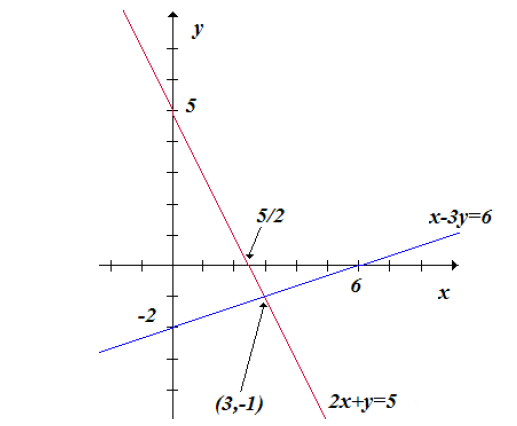
\includegraphics[scale=0.6]{s1}
	\caption{Solução do sistema do Exemplo 01}
	\label{s1}
\end{figure}

\textbf{Exemplo 02: }
Analise o seguinte sistema de equação linear.
$$
\left\{
\begin{array}{c}
2x + y = 5 \\
6x + 3y = 15 \\
\end{array}
\right.
$$
A solução do sistema é $x = -\frac{1}{2}y+\frac{5}{2}$ e $y = \lambda \in \mathbb{R}$.

Como o sistema tem infinitas soluções, estas são representadas pela intersecção das
retas cujas equações gerais são: $2x + y = 5$ e $6x + 3y = 15$ (retas coincidentes).

\begin{figure}[!h]
	\centering
	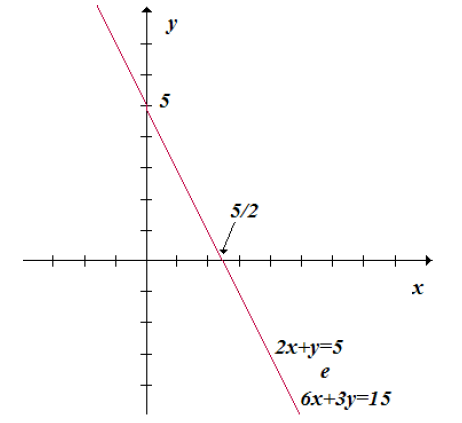
\includegraphics[scale=0.6]{s2}
	\caption{Solução do sistema do Exemplo 02}
	\label{s2}
\end{figure}

\textbf{Exemplo 03: }
Analise o seguinte sistema de equação linear.
$$
\left\{
\begin{array}{c}
2x + y = 5 \\
6x + 3y = 10 \\
\end{array}
\right.
$$

O sistema não tem solução. De fato, as retas cujas equações gerais são: $2x+y=5$ e $6x+3y=10$ são paralelas (não coincidentes).

\begin{figure}[!h]
	\centering
	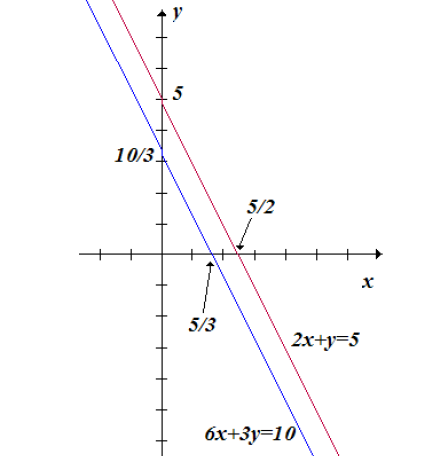
\includegraphics[scale=0.6]{s3}
	\caption{Solução do sistema do Exemplo 03}
	\label{s3}
\end{figure}


No caso de sistemas lineares com mais de duas incógnitas as equações representam planos e outras figuras geométricas. A solução existirá na interseção destes planos.

Considere o seguinte sistema de equações lineares com três incógnitas.

$$
\left\{
\begin{array}{c}
a_{11}x_1 + a_{12}x_2 + a_{13}x_3=b_1 \\
a_{21}x_1 + a_{22}x_2 + a_{23}x_3=b_2 \\
a_{31}x_1 + a_{n2}x_2 + a_{33}x_3=b_3 \\
\end{array}
\right.
$$

cada equação representa um plano no espaço tridimensional. Desta forma os planos $\pi_1$, $\pi_2$ e $\pi_3$ são os planos definidos pelas equações do sistema. Assim, as soluções do referido sistema pertencem à interseção destes planos, isto é, $\pi_1 \cap \pi_2 \cap \pi_3$.

Se pelo menos dois desses planos são paralelos, ou se dois deles intersectam o terceiro segundo retas paralelas, a interseção $\pi_1 \cap \pi_2 \cap \pi_3$ é vazia e o sistema é impossível.

Se os três planos se intersectam em uma reta $r$, isto é, se $\pi_1 \cap \pi_2 \cap \pi_3 = r$, o sistema é indeterminado e qualquer ponto da reta $r$ é uma solução do sistema.

O sistema é determinado (solução única), quando os três planos se encontram em um único ponto.

Existem ao todo, oito posições relativas possíveis para os planos $\pi_1$, $\pi_2$ e $\pi_3$. Quatro dessas posições correspondem aos sistemas impossíveis e nas outras quatro, o sistema tem
solução.

\begin{enumerate}
	\item [Caso 1:] Os três planos coincidem. Neste caso o sistema é indeterminado e qualquer ponto dos planos é uma solução do sistema. \\
	\textbf{Exemplo: }
	
	$
	\left\{
	\begin{array}{c}
	x + 2y - z = 3 \\
	2x+ 4y - 2z = 6 \\
	3x+ 6y - 3z = 9 \\
	\end{array}
	\right.
	$
	
	\item[Caso 2:] Dois planos coincidem e o terceiro é paralelo a eles. Neste caso o sistema é impossível. \\
	\textbf{Exemplo: }
	
	$
	\left\{
	\begin{array}{c}
	x + 2y - z = 3 \\
	2x+ 4y - 2z = 6 \\
	3x+ 6y - 3z = 8 \\
	\end{array}
	\right.
	$
	
	\item [Caso 3:] Dois dos planos coincidem e o terceiro os intersecta segundo uma reta $r$. Neste caso	o sistema é indeterminado e qualquer ponto da reta $r$ é uma solução do sistema. \\
	\textbf{Exemplo: }
	
	$
	\left\{
	\begin{array}{c}
	x + 2y - z = 3 \\
	2x+ 4y - 2z = 6 \\
	3x+ 6y + z = 9 \\
	\end{array}
	\right.
	$
	
	\item [Caso 4:] Os três planos são paralelos dois a dois. Neste caso o sistema é impossível. \\
	\textbf{Exemplo: }

	$
	\left\{
	\begin{array}{c}
	x + 2y - z = 3 \\
	2x+ 4y - 2z = 4 \\
	3x+ 6y - 3z = 5 \\
	\end{array}
	\right.
	$	
	
	\item [Caso 5:] Os planos $\pi_1$ e $\pi_2$ são paralelos e o plano $\pi_3$ os intersecta segundo duas retas paralelas. Neste caso o sistema é impossível. \\
	\textbf{Exemplo: }
	
	$
	\left\{
	\begin{array}{c}
	x + 2y - z = 3 \\
	2x+ 4y - 2z = 4 \\
	x+ 2y + z = 9 \\
	\end{array}
	\right.
	$
	
	\item [Caso 6:] Os três planos são distintos e tem uma reta $r$ em comum, isto é $\pi_1 \cap \pi_2 \cap \pi_3 = r$. Neste caso o sistema é indeterminado e qualquer ponto da reta $r$ é uma solução do sistema. \\
	\textbf{Exemplo: }
	
	$
	\left\{
	\begin{array}{c}
	x + y + z = 1 \\
	2x- y + z = 3 \\
	5x+ 2y + 4z = 6 \\
	\end{array}
	\right.
	$
	
	\item [Caso 7:] Os três planos se intersectam, dois a dois, segundo retas $r = \pi_1 \cap \pi_2$, $s = \pi_1 \cap \pi_3$ e $t = \pi_2 \cap \pi_3$, paralelas umas às outras. Neste caso o sistema é impossível. \\
	\textbf{Exemplo: }

	$
	\left\{
	\begin{array}{c}
	x + 2y - 3z = 1 \\
	3x+ y + z = 2 \\
	8x+ y + 6z = 6 \\
	\end{array}
	\right.
	$	
	
	\item [Caso 8:] Os três planos se intersectam em apenas um ponto. Neste caso, o sistema é possível e determinado (solução única). \\
	\textbf{Exemplo: }

	$
	\left\{
	\begin{array}{c}
	x + 2y + 3z = 1 \\
	2x+ y + z = 2 \\
	3x- y + 2z = 1 \\
	\end{array}
	\right.
	$	
	
\end{enumerate}

\begin{definition}[Forma Escada]
	Uma matriz $m \times n$ é reduzida à forma escada se:
	\begin{enumerate}
		\item O primeiro elemento não nulo de uma linha não nula é $1$;
		\item Cada coluna que contém o primeiro elemento não nulo de alguma linha tem todos os seus outros elementos iguais a zero;
		\item Toda linha nula ocorre abaixo de todas as linhas não nulas (isto é, daquelas que possuem pelo menos um elemento não nulo);
		\item Se as linhas $1, \dots, r$ são as linhas não nulas, e se o primeiro elemento não nulo da linha $i$ ocorre na coluna $k_i$, então $k_1<k_2<\dots<k_r$
	\end{enumerate}
	Essa ultima condição impõe a forma escada à matriz. Ou seja, o número de elementos precedendo o primeiro elemento não nulo de uma linha aumentada a cada linha, até que sobrem somente linhas nulas, se houver.
\end{definition}

\begin{theorem}
	Toda matriz $A_{m \times n}$ é linha equivalente a uma única matriz linha reduzida à forma escada.
\end{theorem}

\begin{definition}[Posto e Nulidade]
	Dada uma matriz $A_{m \times n}$, seja $B_{m \times n}$ a matriz-linha reduzida à forma escada linha equivalente a $A$. O posto de $A$, denotado por $p$, é o número de linhas não nulas de $B$. A nulidade de $A$ é o número $n-p$.
\end{definition}

Dada uma matriz $A$ qualquer, para determinar seu posto é necessário encontrar sua matriz-linha reduzida à forma escada, e depois contar suas linhas não nulas. Este número é o posto de $A$. A nulidade é a diferença entre as colunas de $A$ e o posto.


\begin{theorem}
	\begin{enumerate}
		\item Um sistema de $m$ equações e $n$ incógnitas admite solução se, e somente se, o posto da matriz ampliada é igual ao posto da matriz dos coeficientes.
		\item Se as duas matrizes têm o mesmo posto $p$ e $p=n$, a solução será única.
		\item Se as duas matrizes têm o mesmo posto $p$ e $p<n$, podemos escolher $n-p$ incógnitas, e as outras $p$ incógnitas serão dadas em função destas.
	\end{enumerate}
\end{theorem}

\subsubsection{Sistema de Equações Lineares Homogêneos}

Um sistema linear é homogêneo se os termos independentes são todos nulos, isto é, um sistema da forma $AX=0$. Neste caso, há sempre a solução nula $(x_1,x_2,\dots,x_n)=(0,0,\dots,0)$. Resta ver se tem somente a solução nula (sistema homogêneo determinado) ou se existem outras soluções (sistema homogêneo indeterminado).

Matricialmente, a última coluna da matriz ampliada sendo nula, as operações elementares sobre linhas não modifica essa situação, e por isso, muitas vezes esta coluna é omitida por economia.

Uma relação interessante entre um sistema não homogêneo $AX=B$ e o sistema homogêneo associado $AX=0$, é que se $X_0$ é uma solução particular do sistema não homogêneo, isto é, $AX_0=B$, as outras soluções podem ser escritas na forma $X=X_0+X_1$, onde $X_1$ é uma solução do sistema homogêneo.


\subsubsection{Resolução de Sistemas de Equações Lineares}

\textbf{Método de Escalonamento}
\begin{definition}
	Diz-se que uma matriz é escalonada quando o primeiro elemento não-nulo de cada uma das suas linhas situa-se à esquerda do primeiro elemento não-nulo da linha seguinte. Além disso, as linhas que tiverem todos os seus elementos iguais a zero devem estar abaixo das demais.
\end{definition}

\begin{definition}
	Diz-se que um sistema de equações lineares é um sistema escalonado, quando a matriz aumentada associada a este sistema é uma matriz escalonada. O Método do Escalonamento para resolver ou discutir um sistema de equações lineares $S$ consiste em se obter um sistema de equações lineares escalonado equivalente a $S$ (equivalente no sentido de possuir as mesmas soluções que este).
\end{definition}

Partindo do sistema $S$ pode-se chegar a este sistema escalonado equivalente por meio das operações elementares.

Desta forma, se um sistema de equações foi escalonado e, retiradas as equações do tipo $0=0$, então restam $p$ equações com $n$ incógnitas.

Se a última equação restante é da forma: $0.x_1+0.x_2+\dots+0.x_{n-1}+0.x_n = b_p$ onde $b_p \neq 0$, então o sistema de equações é impossível – S.I. (não admite soluções)

Caso contrário sobram duas opções:
\begin{enumerate}
	\item Se $p=n$ o sistema é possível determinado - S.P.D. (admite solução única).
	\item Se $p<n$, então o sistema é possível indeterminado - S.P.I. (admite infinitas soluções).
\end{enumerate}

\textbf{OBS.}Para se escalonar um sistema S é mais prático efetuar o escalonamento da matriz aumentada associada ao sistema. Uma vez concluído o escalonamento dessa matriz aumentada, associamos a ela o novo sistema que é equivalente ao sistema original $S$.

\textbf{Exemplos}

\textbf{Método de Cramer}

O método de Cramer se aplica para sistemas de equações lineares onde a matriz dos coeficientes das incógnitas é quadrada.

Define-se por $D$ o determinante da matriz dos coeficientes $A$, isto é, $A = \det(A)$ e $D_i$ ao determinante da matriz obtida de $A$, substituindo a {\it i-ésima} coluna pela coluna dos termos independentes.

Assim, se $D \neq 0$, então $x_i = \frac{D_i}{D}$. A solução será única, pois $\exists A^{-1}$ e
\begin{eqnarray*}
A.X &=& B \\
A^{-1}(A.X) &=&A^{-1}.B \\
(A^{-1}.A)X &=&A^{-1}.B \\
I.X &=& A^{-1}.B \\
X &=& A^{-1}.B
\end{eqnarray*}
	
\textbf{OBS 1:} Se $D=D_1=D_2=\dots=D_n=0$ o sistema {\bf não} é necessariamente S.P.I. Utilizar o método de Cramer apenas quando $D \neq 0$.

\textbf{OBS 2:} Embora o método de Cramer apresente de forma explícita a solução do sistema de equações lineares, ele não é muito utilizado para cálculos numéricos. Isto ocorre porque o número de operações que é envolvida é muito grande quando trabalhado com muitas equações.

\textbf{Exemplos}

\subsubsection{Sistemas Lineares - Aplicações}

\newpage
\section{Vetores}

\begin{definition}[Vetores]
	São grandezas que informam a direção, módulo e o sentido.
\end{definition}

\begin{definition}[Segmento Orientado]
	É um par ordenado $(A,B)$ de pontos no espaço. $A$ é a \emph{origem} e $B$ é a \emph{extremidade} do segmento orientado $(A,B)$. Um segmento orientado do tipo $(A,A)$ é chamado \emph{segmento orientado nulo}.
\end{definition}

\begin{definition}
	\begin{enumerate}
		\item Os segmentos orientados $(A,B)$ e $(C,D)$ são \emph{de mesmo comprimento} se os segmentos geométricos $AB$ e $CD$ têm comprimentos iguais.
		\item Se os segmentos orientados $(A,B)$ e $(C,D)$ não são nulos, eles são \emph{de mesma direção} ou \emph{paralelos}, se os segmentos geométricos $AB$ e $CD$ são paralelos (isto inclui o caso em que $AB$ e $CD$ são colineares).
		\item Suponha $(A,B)$ e $(C,D)$ sejam paralelos:
		\begin{itemize}
			\item No caso em que as retas $AB$ e $CD$ são distintas, os segmentos orientados $(A,B)$ e $(C,D)$ são \emph{de mesmo sentido} se os segmentos geométricos tem interseção vazia. Se não, $(A,B)$ e $(C,D)$ são de sentido contrário
			\item No caso em que as retas $AB$ e $CD$ coincidem, tomemos $(E,F)$ tal que $E$ não pertença à reta $AB$, e $(E,F)$ e $(A,B)$ sejam do mesmo sentido, de acordo com o critério anterior. Então, os segmentos orientados $(A,B)$ e $(C,D)$ são \emph{de mesmo sentido} se $(E,F)$ e $(C,D)$ são de mesmo sentido. Se não, $(A,B)$ e $(C,D)$ são \emph{de sentido contrários}.
		\end{itemize}
	\end{enumerate}
\end{definition}

\begin{definition}
	Os segmentos orientados $(A,B)$ e $(C,D)$ são \emph{equipolentes} se forem ambos nulos, ou então, no caso de nenhum deles nulos, possuírem mesma direção, mesmo comprimento e mesmo sentido. Notação: Equipolência entre $(A,B)$ e $(C,D)$ por $(A,B) \sim (C,D)$
\end{definition}

\begin{definition}
	Dado o segmento orientado $(A,B)$, a \emph{classe de equipolência} de $(A,B)$ é o conjunto de todos os segmentos orientados equipolentes a $(A,B)$. O segmento orientado $(A,B)$ é chamado \emph{representante} da classe.
\end{definition}

\begin{definition}[Vetor (formalmente)]
	É uma classe de equipolência de segmentos orientados. Se $(A,B)$ é um segmento orientado, o vetor que tem $(A,B)$ como representante será representado por $\overrightarrow{AB}$. Quando não se quer destacar um representante em especial, usamos letras minúsculas com uma seta $(\overrightarrow{u}, \overrightarrow{v}, \overrightarrow{b}, \dots  )$. O conjunto de todos os vetores será indicado por $\mathbb{V}$. 
\end{definition}

\begin{proposition}
	\begin{enumerate}
		\item É dado um vetor $\overrightarrow{u}$ qualquer. Escolhido arbitrariamente um ponto $P$, existe um segmento orientado representante de $\overrightarrow{u}$ com origem $P$, isto é, existe um ponto $B$ tal que $\overrightarrow{u} = \overrightarrow{PB}$
		\item Tal representante (e, portanto, o ponto $B$) é único, isto é, se $\overrightarrow{PA} = \overrightarrow{PB} \Rightarrow A = B$
	\end{enumerate}
\end{proposition}

\begin{definition}[Vetor Nulo]
	É o vetor que tem como representante um segmento orientado nulo. É indicado por $\overrightarrow{0}$.
\end{definition}

\begin{definition}[Vetor Oposto]
	Se $(A,B)$ é representante de um vetor $\overrightarrow{u}$ o \emph{vetor oposto} de $\overrightarrow{u}$, indicado por $- \overrightarrow{u}$, é o vetor que tem $(B,A)$ como representante. Portanto: $$- \overrightarrow{AB} = \overrightarrow{BA}$$
\end{definition}

\begin{definition}
	\begin{enumerate}
		\item Os vetores $\overrightarrow{u}$ e $\overrightarrow{v}$ são \emph{paralelos} se um representante de $\overrightarrow{u}$ é paralelo a um representante de $\overrightarrow{v}$ (neste caso, qualquer representante de um vetor é paralelo a qualquer representante do outro vetor). {\bf Notação:} $\overrightarrow{u} // \overrightarrow{v}$
		\item Os vetores não nulos e paralelos $\overrightarrow{u}$ e $\overrightarrow{v}$ são \emph{de mesmo sentido} se um representante de $\overrightarrow{u}$ e um de $\overrightarrow{v}$ possuem o mesmo sentido.
		\item Analogamente para o caso de \emph{sentidos opostos}.
		\item O vetor nulo é paralelo a qualquer vetor.
	\end{enumerate}
\end{definition}

\begin{proposition}
	\begin{enumerate}
		\item Se $\overrightarrow{u}$ e $\overrightarrow{v}$ são de mesmo sentido e o mesmo acontece para $\overrightarrow{v}$ e $\overrightarrow{w}$, então $\overrightarrow{u}$ e $\overrightarrow{w}$ são de mesmo sentido.
		\item Se $\overrightarrow{u}$ e $\overrightarrow{v}$ são de sentido contrário e o mesmo acontece para $\overrightarrow{v}$ e $\overrightarrow{w}$, então $\overrightarrow{u}$ e $\overrightarrow{w}$ são de mesmo sentido.
		\item Se $\overrightarrow{u}$ e $\overrightarrow{v}$ são de mesmo sentido e $\overrightarrow{v}$ e $\overrightarrow{w}$ de sentido contrário, então $\overrightarrow{u}$ e $\overrightarrow{w}$ são de sentido contrário.
	\end{enumerate}
\end{proposition}

\begin{definition}[Norma]
	É o comprimento de qualquer um de seus representantes. A norma do vetor $\overrightarrow{u}$ é indicada por $||\overrightarrow{u}||$. Um vetor é \emph{unitário} se sua norma é $1$.
\end{definition}

\begin{proposition}
	Sejam $\overrightarrow{u}$ e $\overrightarrow{v}$ vetores não-nulos. Então $\overrightarrow{u} = \overrightarrow{v}$ se, e somente se, $\overrightarrow{u}$ e $\overrightarrow{v}$ tem normais iguais, são de mesma direção e de mesmo sentido.
\end{proposition}

\newpage

\section{Espaços Vetoriais}

\begin{definition}[Espaço Vetorial]
	Um espaço vetorial real é um conjunto $V$, não vazio, com duas operações:
	\begin{enumerate}
		\item {\bf Soma:} $V \times V \rightarrow V$;
		\item {\bf Multiplicação por Escalar:} $\mathbb{K} \times V \rightarrow V$
	\end{enumerate}
	tais que, para quaisquer $u,v$ e $w \in V$ e $a$ e $b \in \mathbb{K}$, as seguintes propriedades são validas:
	\begin{enumerate}
		\item $(u+v) + w = u + (v + w)$;
		\item $u + v = v + u$;
		\item $\exists 0 \in V; u + 0 = u$ ($0$ é chamado vetor nulo);
		\item $\exists -u \in V; u + (-u) = 0$;
		\item $a(u + v) = au + av$;
		\item $(a + b)v = av + bv$;
		\item $(ab)v = a(bv)$;
		\item $1u = u$.
	\end{enumerate}
\end{definition}

{\bf Exemplo 01:} O conjunto dos vetores do espaço.
$$V = \mathbb{R}^3 = \{ (x_1, x_2, x_3); x_i \in \mathbb{R}\}$$
é um espaço vetorial real.

{\bf Exemplo 02:} O conjunto dos vetores $n-uplas$ de números reais.
$$V = \mathbb{R}^n = \{ (x_1, x_2, \dots, x_n); x_i \in \mathbb{R}\}$$

\emph{Mostrando que realmente é um espaço vetorial.}

\vspace{100pt}

{\bf Exemplo 03:} O conjunto das matrizes reais $m \times n$ com a soma e produto por escalar usuais.

{\bf Exemplo 04:} O conjunto dos polinômios com coeficientes reais, de grau menor ou igual a $n$ (incluindo o zero).

{\bf Exemplo 05:} O conjunto das matrizes $2 \times 2$, cujos elementos são números complexos.

\subsection{Subespaços Vetoriais}

As vezes, é necessário detectar, dentro de um espaço vetorial $V$, subconjuntos $W$ que sejam eles próprios espaços vetoriais ``menores''. Tais conjuntos serão chamados de \emph{subespaços} de $V$.

{\bf Exemplo 01:} $V = \mathbb{R}^2$, o plano, onde $W$ é uma reta deste plano, que passa pela origem.

Note que a reta $W$ funciona sozinha como um espaço vetorial pois, ao somarmos dois vetores de $W$, obtemos outro vetor de $W$, igualmente se multiplicarmos um vetor de $W$ por um escalar.

Em outras palavras, o conjunto $W$ é ``fechado'' em relação à soma de vetores e a multiplicação por escalar.

\begin{definition}[Subespaço Vetorial]
	Dado um espaço vetorial $V$, um subconjunto $W$, não vazio, será um \emph{subespaço vetorial} de $V$ se:
	\begin{enumerate}
		\item Para quaisquer $u,v \in W$ tivermos $u + v \in W$;
		\item Para quaisquer $a \in \mathbb{K}$, $u \in W$ tivermos $au \in W$
	\end{enumerate}
\end{definition}

{\bf OBS.} 
\begin{itemize}
	\item As condições acima garantem que ao operarmos em $W$ (soma e multiplicação por escalar) não obteremos um vetor fora de $W$. É suficiente para afirmar que $W$ é um espaço vetorial, pois as operações estão bem definidas, e não é necessário verificar as condições de espaço vetorial, pois já são validas em $V$, que contém $W$.
	\item Qualquer subespaço $W$ de $V$ necessita conter o vetor nulo (devido a condição 2, no caso de $a=0$).
	\item Todo espaço vetorial admite pelo menos dois subespaços (subespaços triviais), o conjunto formado somente pelo vetor nulo e o próprio espaço vetorial.
\end{itemize}

{\bf Exemplo 01:} $V = \mathbb{R}^3$ e $W \subset V$, um plano passando pela origem.

{\bf Exemplo 02:} $V = \mathbb{R}^5$ e $W = \{(0,x_2, x_3, x_4, x_5); x_i \in \mathbb{R} \}$

\emph{Mostrando que realmente é um subespaço vetorial.}

\vspace{50pt}

{\bf Exemplo 03:} $V = \mathbb{M}(n,m)$ e $W$ é o subconjunto das matrizes triangulares superiores.

{\bf Exemplo 04:}Uma situação importante em que aparece um subespaço é obtida ao resolvermos um sistema linear homogêneo. Por exemplo:

$
\begin{cases}
2x + 4y + z = 0 \\
x + y + 2z = 0 \\
x + 3y - z = 0
\end{cases}
$

\emph{Mostrando que realmente é um subespaço vetorial.}
\vspace{50pt}

{\bf Exemplo 05:} O conjunto-solução de um sistema linear homogêneo de $n$ incógnitas é um subespaço vetorial de $\mathbb{M}(n,1)$.

Exemplos de conjuntos que não são subespaços vetoriais.

{\bf Exemplo 06:} $V = \mathbb{R}^2$, onde $W$ é uma reta deste plano que não passa pela origem.

\emph{Mostrando que $W$ não é um subespaço vetorial.}
\vspace{50pt}

{\bf Exemplo 07:} $V = \mathbb{R}^2$ e $W = \{(x,x^2); x \in \mathbb{R}\}$.

\emph{Mostrando que $W$ não é um subespaço vetorial.}
\vspace{50pt}

{\bf Exemplo 08:} $V = \mathbb{M}(n,n)$ e $W$ é o subconjunto de todas as matrizes em que $a_{11} \leq 0$. Basta mostrar que a condição $2$ não é satisfeita.

\begin{theorem}[Interseção de subespaços]
	Dados $W_1$ e $W_2$ subespaços de um espaço vetorial $V$, a interseção $W_1 \cap W_2$ ainda é um subespaço de $V$.
\end{theorem}

\emph{Prova do Teorema.}
\vspace{50pt}

{\bf Exemplo 01:} $V = \mathbb{M}(n,n)$ e 

$W_1$ = {matrizes triangulares superiores};

$W_2$ = {matrizes triangulares inferiores} e então $W_1 \cap W_2$ = {matrizes diagonais}.

O teorema não é valido para o caso da união de subespaços. Veja o próximo contra-exemplo.

{\bf Exemplo 01:} $V = \mathbb{R}^3$ e $W_1$ e $W_2$ são retas que passam pela origem.

\emph{Mostrando que não é subespaço vetorial.}
\vspace{50pt}

\begin{theorem}[Soma de subespaços]
	Sejam $W_1$ e $W_2$ subespaços de um espaço vetorial $V$. Então, o conjunto
	$$W_1 + W_2 = \{v \in V; v = w_1 + w_2, w_1 \in W_1 \text{ e } w_2 \in W_2 \}$$
	é subespaço de $V$.
\end{theorem}

{\bf Exemplo 01:} O exemplo anterior, $W = W_1 + W_2$ é o plano que contém as duas retas.

{\bf Exemplo 02:} Se $W_1 \subset \mathbb{R}^3$ é um plano e $W_2$ é uma reta contida neste plano, ambos passando pela origem, $W_1 + W_2 = W_1$.

{\bf Exemplo 03:} $W_1 = \left[
\begin{array}{cc}
	a	&	b	\\
	0	&	0	\\
\end{array}
\right]
$
 e $W_2 = \left[
 \begin{array}{cc}
 0	&	0	\\
 c	&	d	\\
 \end{array}
 \right]
 $
, onde $a,b,c,d \in \mathbb{R}$. Então $W_1 + W_2 = \left[
\begin{array}{cc}
a	&	b	\\
c	&	d	\\
\end{array}
\right]
= \mathbb{M}(2,2)
$

Quando $W_1 \cap W_2 = \{0\}$, então $W_1 + W_2$ é chamada \emph{soma direta} de $W_1$ com $W_2$, denotada por $W_1 \oplus W_2$. O exemplo $03$ é um exemplo de soma direta. O exemplo $01$ das matrizes triangulares não é uma soma direta.

\subsection{Combinação Linear}
\begin{definition}
	Sejam $V$ um $\mathbb{K}$-espaço vetorial, $v_1, v_2, \dots, v_n \in V$ e $a_1, \dots, a_n$ escalares. Então, o vetor:
	$$v = a_1 v_1 + a_2 v_2 + \dots + a_n v_n$$
	é um elemento de $V$ ao que chamamos \emph{combinação linear} de $v_1, \dots, v_n$.
\end{definition}

Uma vez fixado os vetores $v_1, \dots, v_n$ em $V$, o conjunto $W$ de todos os vetores de $V$ que são combinações lineares destes, é um subespaço vetorial. {\bf (MOSTRE)}.

$W$ é chamado \emph{subespaço gerado} por $v_1, \dots, v_n$ e usamos a notação
$$W = [v_1, \dots, v_n]$$
Formalmente,
$$W = [v_1, \dots, v_n] = \{ v \in V; v = a_1 v_1 + a_2 v_2 + \dots + a_n v_n, a_i \in \mathbb{R}, 1 \leq i \leq n   \}$$

Outra definição é a seguinte: $W = [v_1, \dots, v_n]$ é o menor subespaço de $V$ que contém o conjunto de vetores $\{ v_1, \dots, v_n \}$, no sentido de que qualquer outro subespaço $W'$ de $V$ que contenha $\{ v_1, \dots, v_n \}$ satisfará $W' \supset W$.

{\bf Exemplo 01:} Se $v_1 , v_2 \in \mathbb{R}^3$ são tais que $\alpha v_1 \neq v_2$ para todo $\alpha \in \mathbb{R}$, então $[v_1, v_2]$ será o plano que passa pela origem e contém $v_1$ e $v_2$.

{\bf Exemplo 02:} $V = \mathbb{R}^2$, $v_1 = (1,0), v_2 = (0,1)$. Logo $V = [v_1 , v_2]$ pois, dado $v = (x,y) \in V$, temos $(x,y) = x(1,0) + y(0,1)$, ou seja, $v = xv_1 + yv_2$.

\subsection{Dependência e Independência Linear}

É de grande importância determinar se um vetor é ou não combinação linear de outros vetores.

\begin{definition}
	Sejam $V$ um espaço vetorial e $v_1 , \dots, v_n \in V$. Dizemos que o conjunto $\{ v_1, \dots, v_n \}$ é \emph{linearmente independente} (LI), ou que os vetores $v_1, \dots, v_n$ são LI, se a equação
	$$a_1 v_1 + \dots + a_n v_n = 0$$
	implica que $a_1 = a_2 = \dots = a_n = 0$. No caso em que exista algum $a_i \neq 0$ dizemos que $\{ v_1, \dots, v_n \}$ é \emph{linearmente dependente} (LD), ou que os vetores $v_1, \dots, v_n$ são LD.
\end{definition}


\begin{theorem}
	$\{ v_1, \dots, v_n \}$ é LD se, e somente se um destes vetores for uma combinação linear dos outros.
\end{theorem}

Equivalentemente, um conjunto de vetores é LI se, e somente se nenhum deles for uma combinação linear dos outros.

{\bf Exemplo 01:} De modo análogo, vemos que para $V = \mathbb{R}^3$, $e_1 = (1,0,0), e_2 = (0,1,0)$ e $e_3 = (0,0,1)$. Então $e_1 , e_2 , e_3$ são LI.

\subsection{Base de um Espaço Vetorial}

Estamos interessados em encontrar, dentro de um espaço vetorial $V$, um conjunto finito de vetores, tais que qualquer outro vetor de $V$ seja uma combinação linear deles. Ou seja, queremos determinar um conjunto de vetores que gere $V$ e tal que todos os elementos sejam realmente necessários para geral $V$. Denominaremos tal conjunto por \emph{base.}

\begin{definition}
	Um conjunto $\{ v_1, \dots, v_n \}$ de vetores de $V$ será uma \emph{base} de $V$ se:
	\begin{itemize}
		\item $\{ v_1, \dots, v_n \}$ é LI;
		\item $[v_1, \dots, v_n] = V$
	\end{itemize}
\end{definition}

{\bf Exemplo 01:} $V = \mathbb{R}^{n}$, $e_1 = (1,0,\dots,0), e_2 = (0,1,0, \dots, 0), \dots, e_n = (0, 0, \dots, 1)$ é base de $V$, conhecida como \emph{base canônica} de $\mathbb{R}^n$.

{\bf Exemplo 02:} O conjunto $\{ (1,1), (0,1) \}$ também é uma base de $V = \mathbb{R}^2$.

\vspace{50pt}
\emph{Mostrando que é base.}

{\bf Exemplo 03:} $V = \mathbb{M}(2,2)$ e $\left[
\begin{array}{cc}
1	&	0	\\
0	&	0	\\
\end{array}
\right]
$, 
$\left[
\begin{array}{cc}
0	&	1	\\
0	&	0	\\
\end{array}
\right]
$,
$\left[
\begin{array}{cc}
0	&	0	\\
1	&	0	\\
\end{array}
\right]
$,
$\left[
\begin{array}{cc}
0	&	0	\\
0	&	1	\\
\end{array}
\right]
$
é uma base de $V$.


\begin{theorem}
	Sejam $v_1, v_2, \dots, v_n$ vetores não nulos que geram um espaço vetorial $V$. Então, dentre estes vetores podemos extrair uma base de $V$.
\end{theorem}

\begin{theorem}
	Seja um espaço vetorial $V$ gerado por um conjunto finito de vetores $v_1, v_2, \dots, v_n$. Então, qualquer conjunto com mais de $n$ vetores é necessariamente LD (e, portanto, qualquer conjunto LI tem no máximo $n$ vetores).
\end{theorem}

\begin{corollary}
	Qualquer base de um espaço vetorial tem sempre o mesmo número de elementos. Este número é chamado \emph{dimensão de} $V$, e denotado \emph{dim}$V$.
\end{corollary}

{\bf Exemplos:} Analisar os exemplos anteriores para determinar a dim$V$.

{\bf OBS.} Quando um espaço vetorial $V$ admite uma base finita, dizemos que $V$ é um espaço de dimensão finita.

\begin{theorem}
	Qualquer conjunto de vetores LI de um espaço vetorial $V$ de dimensão finita pode ser completado de modo a formar uma base de $V$.
\end{theorem}

\begin{corollary}
	Se \emph{dim}$V = n$, qualquer conjunto de $n$ vetores LI formará uma base de V.
\end{corollary}

\begin{theorem}
	Se $U$ e $W$ são subespaços de um espaço vetorial $V$ que tem dimensão finita, então \emph{dim}$U \leq $ \emph{dim}$V$ e \emph{dim}$W \leq $ \emph{dim}$V$. Alem disso,
	$$\dim(U + W) = \dim U + \dim W - \dim(U \cap W)$$
\end{theorem}

\begin{theorem}
	Dada uma base $B = \{ v_1, v_2, \dots, v_n \}$ de $V$, cada vetor de $V$ é escrito de maneira única como combinação linear de $v_1, v_2, \dots, v_n$.
\end{theorem}

\begin{definition}
	Sejam $B = \{ v_1, \dots, v_n \}$ base de $V$ e $v \in V$ onde $v = a_1 v_1 + \dots + a_n v_n$. Chamamos estes números $a_1, a_2, \dots, a_n$ de coordenadas de $v$ em relação à base $B$ e denotamos por:
	$$[v]_B = \left[
	\begin{array}{c}
	a_1	\\
	\vdots	\\
	a_n \\
	\end{array}
	\right]$$
\end{definition}

{\bf Exemplo 01:} Se $B = \{ (1,1), (0,1) \}$, então $(4,3) = x(1,1) + y(0,1)$, resultando em $x = 4$ e $y = -1$.

Então $(4,3) = 4(1,1) -1(0,1)$, donde $[(4,3)]_B = \left[
\begin{array}{c}
4	\\
-1 \\
\end{array}
\right]$

{\bf OBS. } É importante notar que a ordem dos elementos de uma base também influi na matriz das coordenadas de um vetor em relação a esta base.

Por exemplo, se tivermos: $B_1 = \{ (1,0), (0,1) \}$ e $B_2 = \{ (0,1), (1,0) \}$ então

$[(4,3)]_{B1} = \left[
\begin{array}{c}
4	\\
3 \\
\end{array}
\right]$ mas 
$[(4,3)]_{B2} = \left[
\begin{array}{c}
3	\\
4 \\
\end{array}
\right]$

Devido a isso, a partir de agora, sempre que considerarmos uma base $B = \{ v_1, \dots, v_n \}$, estaremos subentendendo que a base seja ordenada na ordem que aparece os vetores.

{\bf Exemplo:} Considere:
$$V = \{ (x,y,z); x + y - z = 0 \}$$
$$W = \{ (x,y,z); x = y \}$$
Determine $V + W$.

\vspace{50pt}
\emph{Resolvendo o exemplo.}

\subsection{Mudança de Base}

A mudança de base tem como objetivo facilitar as operações.
Nosso interesse é na seguinte situação:

Sejam $B = \{ u_1, \dots, u_n \}$ e $B' = \{ w_1, \dots, w_n \}$ duas bases ordenadas de um mesmo espaço vetorial $V$. Dado um vetor $v \in V$, podemos escrevê-lo como:
\begin{eqnarray}
v = x_1 u_1 + \dots + x_n u_n \\
v = y_1 w_1 + \dots + y_n w_n
\end{eqnarray}
Podemos relacionar as coordenadas de $v$ em relação à base $B$,
$$[v]_B = \left[
\begin{array}{c}
x_1	\\
\vdots	\\
x_n \\
\end{array}
\right]$$
e também podemos relacionar as coordenadas de $v$ em relação à base $B'$,
$$[v]_{B'} = \left[
\begin{array}{c}
y_1	\\
\vdots	\\
y_n \\
\end{array}
\right]$$
Como $\{ u_1, \dots, u_n\}$ é base de $V$, podemos escrever os vetores $w_1$ como combinação linear dos $u_j$, isto é,
\begin{eqnarray}
\label{eq01}
\begin{cases}
w_1 = a_{11}u_1 + a_{21}u_2 + \dots + a_{n1}u_n \\
w_2 = a_{12}u_1 + a_{22}u_2 + \dots + a_{n2}u_n \\
\vdots \hspace{40pt} \vdots \hspace{40pt} \vdots \hspace{60pt} \vdots \\
w_n = a_{1n}u_1 + a_{2n}u_2 + \dots + a_{nn}u_n \\
\end{cases}
\end{eqnarray}

\newpage
.
\newpage
A matriz $[I]_{B}^{B'}$ é chamada \emph{matriz de mudança de base $B'$ para a base $B$}.

Compare $[I]_{B}^{B'}$ com (\ref{eq01}) e observe que esta matriz é obtida, colocando as coordenadas em relação a $B$ de $w_i$ na i-ésima coluna. Uma vez obtida $[I]_{B}^{B'}$ podemos encontrar as coordenadas de $v$ na base $B'$ (supostamente conhecidas).

{\bf Exemplo:} Sejam $B = \{ (2,-1), (3,4) \}$ e $B' = \{ (1,0), (0,1) \}$ bases de $\mathbb{R}^2$. Determine $[I]_{B}^{B'}$.

\vspace{50pt}
\emph{Resolvendo o exemplo.}

O cálculo utilizando a matriz de mudança de base é operacionalmente vantajoso quando trabalhamos com mais vetores, pois não há necessidade de resolução de mais de um sistema de equação para cada vetor.

\subsubsection{A inversa da Matriz de Mudança de Base} 
Um fato importante é que as matrizes $[I]_{B}^{B'}$ e $[I]_{B'}^{B}$ são inversíveis e
$([I]_{B}^{B'})^{-1}$ = $[I]_{B'}^{B}$

{\bf Exemplo: } Consideremos em $\mathbb{R}^2$ a base $B = \{ e_1, e_2 \}$ e a base $B' = \{ f_1, f_2 \}$, obtida da base canônica $B$ pela rotação de um ângulo $\theta$. Determine $[I]_{B}^{B'}$.

\vspace{50pt}
\emph{Resolvendo o exemplo.}

\newpage
\section{Transformações Lineares}

\begin{definition}[Transformação Linear]
	Sejam $V$ e $W$ dois espaços vetoriais. Uma \emph{transformação linear} (aplicação linear) é uma função de $V$ em $W$, $T : V \rightarrow W$, que satisfaz as seguintes condições:
	\begin{enumerate}
		\item Quaisquer que sejam $u$ e $v$ em $V$,
		$$T(u + v) = T(u) + T(v)$$
		\item Quaisquer que sejam $\lambda \in \mathbb{R}$ e $v \in V$,
		$$T(\lambda v) = \lambda T(v)$$
	\end{enumerate}
\end{definition}

\subsection{Exemplos de Transformações Lineares}

\begin{enumerate}
	\item $V = \mathbb{R}$ e $W = \mathbb{R}$, onde $T: \mathbb{R} \rightarrow \mathbb{R}$ dada por $T(u) = \alpha u$;
	\\ \emph{Mostrando que é Transformação Linear}
	\\ \vspace{150pt}
	\item $T: \mathbb{R} \rightarrow \mathbb{R}$ dada por $T(u) = u^2$;
	\\ \emph{Mostrando que não é Transformação Linear}
	\\ \vspace{150pt}
	\item $V = \mathbb{R}^2$ e $W = \mathbb{R}^3$, onde $T: \mathbb{R}^2 \rightarrow \mathbb{R}^3$ dada por $T(x,y) = (2x,0,x+y)$;
	\\ \emph{Mostrando que é Transformação Linear}
	\\ \vspace{200pt}
	\\ {\bf OBS.} Da definição de Transformação Linear, $T:V \rightarrow W$ leva o vetor nulo de $V$ no vetor nulo de $W$, isto é, se $0 \in V, T(0) = 0 \in W$. Isto é, se $T(0) \neq 0$ então $T$ não é Transformação Linear. {\bf CUIDADO!} $T(0) = 0$ não implica em $T$ ser linear, ver exemplo 02 anterior.
	\item A aplicação nula.
	\item $V = W = \mathbb{P}_n$, onde $D: \mathbb{P}_n \rightarrow \mathbb{P}_n$ dada por $D(f) = f'$ (aplicação derivada);
	\\ \emph{Mostrando que é Transformação Linear}
	\\ \vspace{200pt}
	\\ O próximo exemplo é um caso particular do seguinte resultado, a toda matriz $m \times n$ está associada uma transformação linear de $\mathbb{R}^n$ em $\mathbb{R}^m$. Isto é, uma matriz produz uma transformação linear, e a recíproca também é verdade, isto é, uma transformação linear produz uma matriz.
	\item $V = \mathbb{R}^n$ e $W = \mathbb{R}^m$, onde $T: \mathbb{R}^n \rightarrow \mathbb{R}^m$, seja $A$ uma matriz $m \times n$. Definimos $L_{A}:\mathbb{R}^n \rightarrow \mathbb{R}^m$ por $L_{A}(v) = A v$, onde $v$ é um vetor coluna de tamanho $n$;
	\\ \emph{Mostrando que é Transformação Linear}
	\\ \vspace{250pt}
\end{enumerate}

\subsection{Transformações do Plano no Plano}
Os seguintes exemplos são para ilustrar geometricamente as transformações lineares no plano $\mathbb{R}^2$.

\subsubsection{Exemplos de Transformações no Plano}
\begin{enumerate}
	\item {\bf Expansão (ou Contração) Uniforme:} $T:\mathbb{R}^2 \rightarrow \mathbb{R}^2$, $\alpha \in \mathbb{R}$ onde $T(v) = \alpha v$. 
	\\ {\bf Exemplo:} $T:\mathbb{R}^2 \rightarrow \mathbb{R}^2$, $\alpha \in \mathbb{R}$ onde $T(v) = 2v$ ou $T(x,y) = 2(x,y)$. Essa função leva cada vetor do plano num vetor de mesma direção e sentido de $v$, mas de módulo maior.
	\vspace{150pt}
	\\ Escrevendo na forma de vetores-coluna,
	\\
	$\left[
	\begin{array}{c}
	x\\
	y \\
	\end{array}
	\right]$ $\rightarrow$ $2 \left[
	\begin{array}{c}
	x\\
	y \\
	\end{array}
	\right]$
	ou 
	$\left[
	\begin{array}{c}
	x\\
	y \\
	\end{array}
	\right]$ $\rightarrow$
	$\left[
	\begin{array}{cc}
	2	&	0\\
	0	&	2 \\
	\end{array}
	\right]$
	$\left[
	\begin{array}{c}
	x\\
	y \\
	\end{array}
	\right]$
	\item {\bf Reflexão em Torno do Eixo $x$:} $F:\mathbb{R}^2 \rightarrow \mathbb{R}^2$, onde $F(x,y) = (x,-y)$. 
	\\ \vspace{150pt}
	\\
	$\left[
	\begin{array}{c}
	x\\
	y \\
	\end{array}
	\right]$ $\rightarrow$ $ \left[
	\begin{array}{c}
	x\\
	-y \\
	\end{array}
	\right]$
	ou 
	$\left[
	\begin{array}{c}
	x\\
	y \\
	\end{array}
	\right]$ $\rightarrow$
	$\left[
	\begin{array}{cc}
	1	&	0\\
	0	&	-1 \\
	\end{array}
	\right]$
	$\left[
	\begin{array}{c}
	x\\
	y \\
	\end{array}
	\right]$
	\item {\bf Reflexão na Origem:} $T:\mathbb{R}^2 \rightarrow \mathbb{R}^2$, onde $F(x,y) = (-x,-y)$. 
	\\ \vspace{150pt}
	\\
	$\left[
	\begin{array}{c}
	x\\
	y \\
	\end{array}
	\right]$ $\rightarrow$ $ \left[
	\begin{array}{c}
	-x\\
	-y \\
	\end{array}
	\right]$
	ou 
	$\left[
	\begin{array}{c}
	x\\
	y \\
	\end{array}
	\right]$ $\rightarrow$
	$\left[
	\begin{array}{cc}
	-1	&	0\\
	0	&	-1 \\
	\end{array}
	\right]$
	$\left[
	\begin{array}{c}
	x\\
	y \\
	\end{array}
	\right]$
	\item {\bf Rotação de um Ângulo $\theta$:} (no sentido anti-horário)
	\\ \vspace{150pt}
	\\ $x' = r \cos(\alpha + \theta) = r \cos(\alpha) \cos(\theta) - r \sin(alpha) \sin(\theta)$
	
	Mas $r\cos(\theta) = x$ e $r\sin(\theta) = y$
	
	Então, $x' = x\cos(\theta) - y\sin(\theta)$
	
	Analogamente, $y' = r \sin(\alpha + \theta) = r(\sin(\alpha) \cos(\theta) + \cos(\alpha)\sin(\theta)) = y\cos(\theta) + x\sin(\theta)$
	
	Assim, $R_{\theta}(x,y) = (x\cos(\theta) - y\sin(\theta), y\cos(\theta) + x\sin(\theta))$ ou na forma coluna,
	
	$\left[
	\begin{array}{c}
	x\\
	y \\
	\end{array}
	\right]$ $\rightarrow$
	$\left[
	\begin{array}{c}
	x\cos(\theta) - y\sin(\theta)\\
	y\cos(\theta) + x\sin(\theta) \\
	\end{array}
	\right] = $
	$\left[
	\begin{array}{cc}
	\cos(\theta)	&	-\sin(\theta)\\
	\sin(\theta)	&	\cos(\theta) \\
	\end{array}
	\right]$
	$\left[
	\begin{array}{c}
	x\\
	y \\
	\end{array}
	\right]$
	
	COnsiderando o caso particular onde $\theta = \frac{\pi}{2}$. Neste caso, $\cos(\theta) = 0$ e $\sin(\theta) = 1$
	
	Então,
	
	$\left[
	\begin{array}{c}
	x\\
	y \\
	\end{array}
	\right]$ $\rightarrow$
	$\left[
	\begin{array}{c}
	-y	\\
	x	\\
	\end{array}
	\right] = $
	$\left[
	\begin{array}{cc}
	0	&	-1\\
	1	&	0 \\
	\end{array}
	\right]$
	$\left[
	\begin{array}{c}
	x\\
	y \\
	\end{array}
	\right]$
	
	\vspace{150pt}
	
	\item {\bf Cisalhamento horizontal:} $T:\mathbb{R}^2 \rightarrow \mathbb{R}^2$, $\alpha \in \mathbb{R}$ onde $T(x,y) = (x + \alpha y, y)$.
	
	Por exemplo, $T(x,y) = (x + 2y, y)$ 
	
	$\left[
	\begin{array}{c}
	x\\
	y \\
	\end{array}
	\right]$ $\rightarrow$
	$\left[
	\begin{array}{c}
	x + 2y	\\
	y	\\
	\end{array}
	\right] = $
	$\left[
	\begin{array}{cc}
	1	&	2\\
	0	&	1 \\
	\end{array}
	\right]$
	$\left[
	\begin{array}{c}
	x\\
	y \\
	\end{array}
	\right]$
	
	
	Um exemplo de Transformação que não é linear.
	\item {\bf Translação:} $T(x,y) = (x + a,y + b)$ ou
	
	$\left[
	\begin{array}{c}
	x\\
	y \\
	\end{array}
	\right]$ $\rightarrow$
	$\left[
	\begin{array}{cc}
	1	&	0	\\
	0	&	1	\\
	\end{array}
	\right]  $
	$\left[
	\begin{array}{c}
	x \\
	y \\
	\end{array}
	\right] + $
	$\left[
	\begin{array}{c}
	a\\
	b \\
	\end{array}
	\right]$
	
\end{enumerate}

\subsection{Conceitos e Teoremas}

\begin{theorem}
	Dados dois espaços vetoriais reais $V$ e $W$ e uma base de $V$, $\{ v_1, v_2, \dots, v_n \}$, sejam $w_1, w_2, \dots, w_n$ elementos arbitrários de $W$. Então existe uma única aplicação linear $T: V \rightarrow W$ tal que $T(v_1) = w_1, \dots, T(v_n) = w_n$. Essa aplicação é dada por:
	
	Se $v = a_1 v_1 + \dots + a_n v_n$,
	\begin{eqnarray*}
		T(v) & = & a_1 T(v_1) + \dots + a_n T(v_n) \\
			& = & a_1 w_1 + \dots + a_n w_n
	\end{eqnarray*}
	
	\emph{Verifique que $T$ assim definida é linear e que é a única que satisfaz as condições exigidas.}
\end{theorem}

{\bf Exemplo 01:} Qual é a transformação linear $T:\mathbb{R}^2 \rightarrow \mathbb{R}^3$ tal que $T(1,0) = (2,-1,0)$ e $T(0,1) = (0,0,1)$?

\vspace{150pt}

Definiremos os conjuntos \emph{núcleo} e \emph{imagem} de uma Transformação Linear.

\begin{definition}[Imagem de uma Transformação Linear]
	Seja $T:V \rightarrow W$ uma aplicação linear. A \emph{imagem} de $T$ é o conjunto dos vetores $w \in W$ tais que existe um vetor $v \in V$, que safisfaz $T(v) = w$. Ou seja,
	$$Im(T) = \{ w \in W; T(v) = w \text{ para algum } v \in V  \}$$
	
	Note que $Im(T)$ é um subconjunto de $W$ e, além disso, é um subespaço vetorial de $W$.
\end{definition}

\begin{definition}[Núcleo de uma Transformação Linear]
	Seja $T:V \rightarrow W$ uma transformação linear. O conjunto de todos os vetores $v \in V$ tais que $T(v) = 0$ é chamado \emph{núcleo} de $T$, sendo denotado por $ker(T)$. Isto é:
	$$ket(T) = \{ v \in V; T(v) = 0 \}$$
	
	Note que $Ker(T) \subset V$ é um subconjunto de $V$ e, além disso, é um subespaço vetorial de $V$.
	
	\vspace{150pt}
\end{definition}

{\bf Exemplo 01:} $T: \mathbb{R}^2 \rightarrow \mathbb{R}$ onde $T(x,y) = x + y$

\vspace{200pt}

{\bf Exemplo 02:} Seja a transformação linear $T: \mathbb{R}^3 \rightarrow \mathbb{R}^3$ dada por $T(x,y,z) = (x,2y,0)$

\vspace{300pt}


Recordaremos as definições de função injetora e sobrejetora para relacionarmos tais conceitos com transformações lineares.

\begin{definition}
	Dada uma aplicação (ou função) $T: V \rightarrow W$, diremos que $T$ é \emph{injetora} se dados $u \in V$, $v \in V$ com $T(u) = T(v)$ tivermos $u = v$. Equivalentemente, $T$ é injetora se dados $u,v \in V$ com $u \neq v$, então $T(u) \neq T(v)$.
	
	Em outras palavras, $T$ é injetora se as imagens de vetores distintos são distintas.
	
	\vspace{100pt}
\end{definition}

\begin{definition}
	A aplicação $T: V \rightarrow W$ será \emph{sobrejetora} se a imagem de $T$ coincidir com $W$, ou seja $T(V) = W$.
	
	Em outras palavras, $T$ será sobrejetora se dado $w \in W$, existir $v \in V$ tal que $T(v) = w$.
	
	\vspace{100pt}
\end{definition}

\begin{theorem}
	Seja $T: V \rightarrow W$, uma aplicação linear. Então $ker(T) = \{0\}$, se e somente se $T$ é injetora.
\end{theorem}
{\bf PROVA:}
\vspace{300pt}

Uma consequência é que uma aplicação linear injetora leva vetores LI em vetores LI.

\begin{theorem}[do Núcleo e Imagem]
	Seja $T:V \rightarrow W$ uma aplicação linear. Então:
	$$dim(V) = dim(ker(T)) + dim(Im(T))$$
\end{theorem}
{\bf PROVA:}
\vspace{400pt}

\begin{corollary}
	Se $dimV = dimW$, então $T$ linear é injetora se e somente se $T$ é sobrejetora.
\end{corollary}

\begin{corollary}
	Seja $T:V \rightarrow W$ uma aplicação linear injetora. Se $dimV = dimW$, então $T$ leva base em base.
\end{corollary}
{\bf PROVA:}
\vspace{200pt}

Quando $T: V \rightarrow W$ for injetora e sobrejetora, ao mesmo tempo, dá-se o nome de \emph{isomorfismo}. Quando há uma tal transformação entre dois espaços vetoriais dizemos que estes são \emph{isomorfos}. 

No ponto de vista da álgebra linear, dois espaços vetoriais \emph{isomorfos} são, por assim dizer, idênticos. Devido aos resultados anteriores, os espaços isomorfos possuem a mesma dimensão e um isomorfismo leva base a base.

Além, disso $T: V \rightarrow W$ tem uma aplicação inversa $T^{-1}:W \rightarrow V$ que é linear {\bf (MOSTRE)} e também é um isomorfismo.

{\bf Exemplo 01: } Seja $T: \mathbb{R}^{3} \rightarrow \mathbb{R}^{3}$ dada por $T(x,y,z) = (x - 2y,z, x+y)$. Mostre que $T$ é isomorfismo e determine $T^{-1}$.
\vspace{250pt}

\subsection{Aplicações Lineares e Matrizes}

Já sabemos que a toda matriz $m \times n$ está associada uma transformação linear $T:\mathbb{R}^n \rightarrow \mathbb{R}^m$. Nesta seção será formalizado para espaços vetoriais $V$ e $W$ e também será estabelecido o recíproco, isto é, uma vez fixadas as bases, toda transformação linear $T: V \rightarrow W$ estará associada uma única matriz.

{\bf Exemplo 01:} Consideramos $\mathbb{R}^2$ e as bases:

$B = \{ (1,0),(0,1) \}$ e $B' = \{ (1,1), (-1,1) \}$ e a matriz $A = $ $\left[
\begin{array}{cc}
2	&	0	\\
0	&	1	\\
\end{array}
\right]  $. Queremos associar a esta matriz $A$ uma aplicação linear que depende de $A$ e das bases dadas $B$ e $B'$, isto é,
$$T_A : \mathbb{R}^2 \rightarrow \mathbb{R}^2$$
$$v \rightarrow T_A (v)$$

\newpage

{\bf Exemplo 02: } $A = $ $\left[
\begin{array}{ccc}
1	&	-3	&	5 \\
2	&	4	&	-1	\\
\end{array}
\right]$, $B = \{ (1,0), (0,1) \}$ e $B' = \{ (1,0,0), (0,1,0), (0,0,1) \}$ e $T_A : \mathbb{R}^3 \rightarrow \mathbb{R}^2$. Determine $T_A$.
\vspace{150pt}

Agora vamos encontrar a matriz associada a uma transformação linear. Seja $T: V \rightarrow W$ linear, $B = \{ v_1, \dots, v_n \}$ base de $V$ e $B' = \{ w_1, \dots, w_m \}$ base de $W$. Então $T(v_1), \dots, T(v_n)$ são vetores de $W$ e portanto

\begin{eqnarray*}
T(v_1) = a_{11}w_1 + a_{21}w_2 + \dots + a_{m1}w_m \\
\vdots \hspace{40pt} \vdots \hspace{40pt} \vdots \hspace{60pt} \vdots \\
T(v_n) = a_{1n}w_1 + a_{2n}w_2 + \dots + a_{mn}w_m \\
\end{eqnarray*}


A transposta da matriz de coeficientes deste sistema, denotada por $[T]_{B'}^{B}$, é chamada matriz de $T$ em relação às bases $B$ e $B'$.

$$ [T]_{B'}^{B} = \left[
\begin{array}{ccc}
a_{11}	&	\dots	&	a_{1n} \\
\vdots	&			&	\vdots	\\
a_{m1}	&	\dots	&	a_{mn}
\end{array}
\right] = A$$

Note que $T$ passa a ser a aplicação linear associada à matriz $A$ e bases $B$ e $B'$, isto é $T = T_A$.

{\bf Exemplo 03:} Seja $T:\mathbb{R}^3 \rightarrow \mathbb{R}^2$ tal que $T(x,y,z) = (2x + y - z, 3x - 2y + 4z)$. Sejam $B = \{ (1,1,1), (1,1,0), (1,0,0) \}$ e $B' = \{ (1,3), (1,4) \}$. Determine $[T]_{B'}^{B}$.
\vspace{150pt}

{\bf OBS.} Se fossem utilizadas outras bases, teríamos outra matriz associada a $T$.

{\bf Exemplo 04: }Dadas as bases $B = \{ (1,1), (0,1) \}$ de $\mathbb{R}^2$ e $B' = \{ (0,3,0), (-1,0,0), (0,1,1) \}$ de $\mathbb{R}^3$, encontremos a transformação linear $T: \mathbb{R}^2 \rightarrow \mathbb{R}^3$ cuja matriz é:
$[T]_{B'}^{B} = \left[
\begin{array}{cc}
0	&	2	\\
-1	&	0	\\
-1	&	3
\end{array}
\right]  $

\vspace{150pt}

\begin{theorem}
	Sejam $V$ e $W$ espaços vetoriais, $\alpha$ base de $V$, $\beta$ base de $W$ e $T: V \rightarrow W$ uma aplicação linear. Então, para todo $v \in V$ vale:
	$$[T(v)]_{\beta} = [T]_{\beta}^{\alpha} \cdot [v]_{\alpha}$$
	\vspace{100pt}
\end{theorem}
Através deste teorema, o estudo de transformações lineares entre espaços de dimensão finita é reduzido ao estudo de matrizes. No caso particular de $V = W$ e $T = I$, o resultado é o mesmo da matriz de mudança de base.

{\bf Exemplo 05:} Seja a transformação linear $T: \mathbb{R}^2 \rightarrow \mathbb{R}^3$ dada por
$$[T]_{\alpha}^{\beta} = \left[
\begin{array}{cc}
1	&	-1	\\
0	&	1	\\
-2	&	3
\end{array}
\right] 
$$
onde $\alpha = \{ (1,0), (0,1) \}$ é base de $\mathbb{R}^2$, $\beta = \{ (1,0,1), (-2,0,1), (0,1,0) \}$ é base de $\mathbb{R}^3$. Qual a imagem do vetor $v = (2,-3)$ gerada por $T$.
\vspace{150pt}

O relacionamento entre as dimensões do núcleo e da imagem de uma transformação linear e o posto de uma matriz associada é dado no teorema a seguir.

\begin{theorem}
	Seja $T:V \rightarrow W$ uma aplicação linear e $\alpha$ e $\beta$ bases de $V$ e $W$ respectivamente. Então:
	
	$$\dim Im(T) =  \text{posto de } [T]_{\beta}^{\alpha}$$
	$$\dim ker(T) = \text{nulidade de } [T]_{\beta}^{\alpha}$$
	
	ou ainda, $\dim ker(T) = $ número de colunas - posto de $[T]_{\beta}^{\alpha}$.
\end{theorem}

\begin{theorem}
	Sejam $T_1 : V \rightarrow W$ e $T_2 : W \rightarrow U$ transformações lineares e $\alpha, \beta$ e $\gamma$ bases de $V, W$ e $U$ respectivamente. Então a composta de $T_1$ com $T_2$, $T_1 \circ T_2: V \rightarrow U$ é linear e
	$$[T_2 \circ T_1]_{\gamma}^{\alpha} = [T_2]_{\gamma}^{\beta} \cdot [T_1]_{\beta}^{\alpha}$$
	\vspace{100pt}
\end{theorem}

{\bf Exemplo 01: } Consideramos uma expansão do plano $\mathbb{R}^2$ dada por $T_1(x,y) = 2(x,y)$, e um cisalhamento dado por $T_2(x,y) = (x+2y,y)$.
\vspace{300pt}

{\bf Exemplo 02: } Sejam as transformações lineares $T_1: \mathbb{R}^2 \rightarrow \mathbb{R}^3$ e $T_2: \mathbb{R}^3 \rightarrow \mathbb{R}^2$ cujas matrizes são:

$$[T_1]_{\beta}^{\alpha} = \left[
\begin{array}{cc}
1	&	0	\\
1	&	-1	\\
0	&	1
\end{array}
\right] 
\text{ e }
[T]_{\gamma}^{\beta} = \left[
\begin{array}{ccc}
	0	&	1	&	-1	\\
	0	&	0	&	0	\\
\end{array}
\right] 
$$
em relação às bases $\alpha = \{ (1,0), (0,2) \}$, $B = \{ (\frac{1}{3},0,-3), (1,1,15), (2,0,5) \}$ e $\gamma = \{ (2,0), (1,1) \}$. Determine a transformação linear composta $T_2 \circ T_1: \mathbb{R}^2 \rightarrow \mathbb{R}^2$, isto é, $(T_2 \circ T_1)(x,y)$.
\vspace{300pt}

\begin{corollary}
	Se $T: V \rightarrow W$ é uma transformação linear inversível ($T$ é um isomorfismo) e $\alpha$ e $\beta$ são bases de $V$ e $W$, então $T^{-1}:W \rightarrow V$ é um operador linear e 
	$$[T^{-1}]_{\alpha}^{\beta} = ([T]_{\beta}^{\alpha})^{-1}$$
	\vspace{100pt}
\end{corollary}

\begin{corollary}
	Seja $T: V \rightarrow W$ uma transformação linear e $\alpha$ e $\beta$ bases de $V$ e $W$. Então $T$ é inversível se e somente se $\det[T]_{\beta}^{\alpha} \neq 0$.
\end{corollary}

{\bf Exemplo 01: } Seja $T: \mathbb{R}^2 \rightarrow \mathbb{R}^2$ uma transformação linear dada por:
$$[T]_{\xi}^{\xi} = \left[
\begin{array}{cc}
3	&	4	\\
2	&	3	\\
\end{array}
\right] 
$$
 onde $\xi$ é a base canônica de $\mathbb{R}^2$. Determine $T^{-1}$.
 
 \begin{corollary}
 	Conhecendo a matriz de uma transformação linear em relação a certas bases $\alpha$ e $\beta$ e as matrizes de mudança de base para novas bases $\alpha'$ e $\beta'$, podemos achar a matriz da mesma transformação linear, desta vez em relação às novas bases $\alpha'$ e $\beta'$. Matematicamente,
 	$$[T]_{\beta'}^{\alpha'} = [I \circ T \circ I]_{\beta'}^{\alpha'} = [I]_{\beta'}^{\beta}[T]_{\beta}^{\alpha}[I]_{\alpha}^{\alpha'}$$
 \end{corollary}
Como caso particular, se $T: V \rightarrow V$ é uma transformação linear e $\alpha$ e $\beta$ são bases de $V$, então
$$[T]_{\beta}^{\beta} = [I \circ T \circ I]_{\beta}^{\beta} = [I]_{\beta}^{\alpha}[T]_{\alpha}^{\alpha}[I]_{\alpha}^{\beta}$$

Lembre-se que $[I]_{\alpha}^{\beta} = ([I]_{\beta}^{\alpha})^{-1}$ denotando $[I]_{\alpha}^{\beta} = A$, segue que

$$[T]_{\beta}^{\beta} = A \cdot [T]_{\alpha}^{\alpha} \cdot A^{-1}$$

Dizemos neste caso que as matrizes $[T]_{\alpha}^{\alpha}$ e $[T]_{\beta}^{\beta}$ são \emph{semelhantes}.

{\bf Exemplo: } Seja a transformação linear $T: \mathbb{R}^3 \rightarrow \mathbb{R}^3$ cuja matriz em relação à base canônica $\xi$ é:

$$[T]_{\xi}^{\xi} = \left[
\begin{array}{ccc}
-2	&	4	&	-4	\\
1	&	-2	&	2	\\
3	&	-6	&	5
\end{array}
\right] 
$$
Calculemos a matriz desta transformação em relação à base $B = \{ (0,1,1), (-1,0,1), (1,1,1) \}$.
\vspace{230pt}

\newpage
\section{Autovalores e Autovetores}

Ao estudarmos conceitos de autovalores e autovetores estaremos interessados em determinar uma classe especial de vetores no espaço vetorial, que satisfaça a propriedade definida. Como forma de introduzir esses conceitos, tomemos os seguintes exemplos.

{\bf Exemplo 01:} Dada $T: V \rightarrow V$, quais vetores $v \in V$ tais que $T(v) = v$? ($v$ é denominado \emph{vetor fixo}).

O primeiro exemplo é o trivial, a aplicação identidade, onde todo vetor é definido como vetor fixo.

{\bf Exemplo 02: } $r_x:\mathbb{R}^2 \rightarrow \mathbb{R}^2$ dada por $r_x (x,y) = (x,-y)$ ou 

$\left[
\begin{array}{c}
x\\
y \\
\end{array}
\right]$ $\rightarrow$
$\left[
\begin{array}{cc}
1	&	0\\
0	&	-1 \\
\end{array}
\right]$
$\left[
\begin{array}{c}
x\\
y \\
\end{array}
\right]$

\vspace{100pt}
Esses vetores são únicos.
\vspace{230pt}



Dada uma transformação linear de um espaço vetorial $T: V \rightarrow V$, nosso interesse é descobrir quais vetores são levados em um múltiplo de si mesmo, isto é, procuramos um vetor $v \in V$ e um escalar $\lambda \in \mathbb{R}$ tais que:
$$T(v) = \lambda v$$.

Neste caso, $T(v)$ será um vetor de mesma ``direção'' que $v$ (sobre a mesma reta suporte). Como $v = 0$ satisfaz a equação para todo $\lambda$, estamos interessados em determinar vetores $v \neq 0$ satisfazendo a condição acima. 

\begin{definition}[Autovetor e Autovalor]
	Seja $T: V \rightarrow V$ um operador linear. Se existirem $v \in V$, $v \neq 0$, e $\lambda \in \mathbb{R}$ tais que $T(v) = \lambda v$, $\lambda$ é um \emph{autovalor} de $T$ e $v$ é um \emph{autovetor} de $T$ associado a $\lambda$.
	
	Note que $\lambda$ pode ser igual a $0$, embora $v \neq 0$.
\end{definition}

{\bf Exemplo 01: } $T: \mathbb{R}^2 \rightarrow \mathbb{R}^2$ onde $T(x,y) = 2(x,y)$

$\left[
\begin{array}{c}
x\\
y \\
\end{array}
\right]$ $\rightarrow$
$\left[
\begin{array}{cc}
2	&	0\\
0	&	2 \\
\end{array}
\right]$
$\left[
\begin{array}{c}
x\\
y \\
\end{array}
\right] = $
$\left[
\begin{array}{c}
2x\\
2y \\
\end{array}
\right] = 2$
$\left[
\begin{array}{c}
x\\
y \\
\end{array}
\right]$

Neste caso, $2$ é um autovalor de $T$ e qualquer $(x,y) \neq (0,0)$ é um autovetor de $T$ associado ao autovalor $2$.
\vspace{130pt}

De modo geral toda transformação do tipo $T: \mathbb{R}^2 \rightarrow \mathbb{R}^2$ onde $T(x,y) = \alpha(x,y), \alpha \neq 0$
tem $\alpha$ como autovalor e qualquer $(x,y) \neq (0,0)$ como autovetor correspondente. Note que $T(v)$ é sempre um vetor de mesma direção que $v$. Ainda mais se,
\begin{enumerate}
	\item $\alpha < 0$, $T$ inverte o sentido do vetor;
	\item $|\alpha| > 1$, $T$ dilata o vetor;
	\item $|\alpha| < 1$, $T$ contrai o vetor;
	\item $\alpha = 1$, $T$ é a identidade
\end{enumerate}

{\bf Exemplo 02: } Seja $A = \left[
\begin{array}{cc}
2	&	2\\
0	&	1 \\
\end{array}
\right]$
\vspace{400pt}

\begin{theorem}
	Dada uma transformação $T:V \rightarrow V$ e um autovetor $v$ associado a um autovalor $\lambda$, qualquer vetor $w = \alpha v (\alpha \neq 0)$ também é um autovetor de $T$ associado a $\lambda$.
\end{theorem}

{\bf MOSTRE QUE:} o conjunto formado pelos autovetores associados a um autovalor $\lambda$ e o vetor nulo é um subespaço vetorial de $V$, isto é, $V_\lambda = \{ v \in V; T(v) = \lambda v \}$ é subespaço de $V$.

\begin{definition}
	O subespaço $V_\lambda = \{ v \in V; T(v) = \lambda v \}$ é chamado o \emph{subespaço associado ao autovalor} $\lambda$.
\end{definition}

\subsection{Autovalores e Autovetores de uma Matriz}

Dada uma matriz quadrada de ordem $n$, $A$, estaremos entendendo por \emph{autovalor} e \emph{autovetor} de $A$, autovalor e autovetor da transformação linear $T_A:\mathbb{R}^n \rightarrow \mathbb{R}^n$, associada à matriz $A$ em relação à base canônica, isto é, $T_A (v) = A \cdot v$ (na forma coluna). Assim, um autovalor $\lambda \in \mathbb{R}$ de $A$, e um autovetor $v \in \mathbb{R}^n$, são soluções da equação $A \cdot v = \lambda v, v \neq 0$.

{\bf Exemplo 01:} Dada a matriz diagonal
$$A = \left[
\begin{array}{cccc}
a_{11}	&	0		&	\dots	&	0\\
0		&	a_{22}	&	\dots	&	0 \\
\vdots	&	\vdots	&			&	\vdots	\\
0		&	0		&	\dots	&	a_{nn}
\end{array}
\right]$$
e dados os vetores da base canônica de $\mathbb{R}^n$, temos
$$A \cdot e_1 = \left[
\begin{array}{c}
a_{11}\\
0 \\
\vdots \\
0
\end{array}
\right] = a_{11}e_1$$
e em geral, $A \cdot e_i = a_{ii}e_i$. Então, estes vetores da base canônica de $\mathbb{R}^n$ são autovetores para $A$, e o autovetor $e_i$ é associado ao autovalor $a_{ii}$.

A próxima seção mostrará que dada uma transformação linear $T: V \rightarrow V$ e fixada uma base $B$ podemos reduzir o problema de encontrar autovalores e autovetores para $T$ à determinação de autovalores para a matriz $[T]_{B}^{B}$.

\subsection{Polinômio Característico}

Nesta seção determinaremos um método prático para determinar autovalores e autovetores de uma matriz real $A$ de ordem $n$.

Inicialmente tomaremos um exemplo onde $n=3$ e depois será generalizado para $n$ qualquer.

{\bf Exemplo: }
$$A = \left[
\begin{array}{ccc}
4	&	2	&	0\\
-1	&	1	&	0 \\
0	&	1	&	2	\\
\end{array}
\right]$$
Nosso interesse esta em determinar vetores $v \in \mathbb{R}^3$ e escalares $\lambda \in \mathbb{R}$ tais que $A \cdot v = \lambda v$.

Observe que se $I$ for a matriz identidade de ordem $3$, então a equação acima pode ser escrita na forma $Av = (\lambda I)v$, ou ainda, $(A - \lambda I)v = 0$.

Escrevendo explicitamente, temos:
$$\left( \left[
\begin{array}{ccc}
4	&	2	&	0\\
-1	&	1	&	0 \\
0	&	1	&	2	\\
\end{array}
\right] - \left[
\begin{array}{ccc}
\lambda	&	0		&	0\\
0		&	\lambda	&	0 \\
0		&	0		&	\lambda	\\
\end{array}
\right] \right) \left[
\begin{array}{c}
x	\\
y	\\
z	\\
\end{array}
\right] = 
\left[
\begin{array}{c}
0	\\
0	\\
0	\\
\end{array}
\right]$$

Disso temos a seguinte equação matricial:

$$\left[
\begin{array}{ccc}
4 - \lambda	&	2	&	0\\
-1	&	1 - \lambda	&	0 \\
0	&	1	&	2 - \lambda	\\
\end{array}
\right] \left[
\begin{array}{c}
x	\\
y	\\
z	\\
\end{array}
\right] = \left[
\begin{array}{c}
0	\\
0	\\
0	\\
\end{array}
\right]$$

Escrevendo o sistema de equações lineares equivalente a esta equação matricial, obteremos um sistema de três equações e três incógnitas.

Se o determinante da matriz dos coeficientes foi igual a 0, implica que o sistema só possuíra uma única solução, neste caso a solução trivial, ou seja, $x=y=z=0$. Como nosso interesse é calcular os autovetores de $A$, isto é, $v \neq 0$, tais que $(A - \lambda I)v = 0$ Assim, neste caso $\det(A - \lambda I)$ deve ser zero.

$$\left[
\begin{array}{ccc}
4 - \lambda	&	2	&	0\\
-1	&	1 - \lambda	&	0 \\
0	&	1	&	2 - \lambda	\\
\end{array}
\right] = 0 $$

E portanto, $-\lambda ^3 + 7 \lambda ^2 - 16 \lambda + 12 = 0$. Vemos que $\det(A - \lambda I)$ é um polinômio em $\lambda$. Este polinômio é chamado o \emph{polinômio característico} de $A$.

Continuando a resolução, temos $(\lambda - 2)^2(\lambda -3) = 0$. Dessa forma, $\lambda = 2$ e $\lambda = 3$ são as raízes do polinômio característico de $A$, e portanto os autovalores da matriz $A$.

Conhecendo os autovalores, podemos determinar os autovetores, resolvendo a equação $Av = \lambda v$, para os casos:
\begin{enumerate}
	\item [i)] $\lambda = 2$
	
	$$\left[
	\begin{array}{ccc}
	4	&	2	&	0\\
	-1	&	1	&	0 \\
	0	&	1	&	2	\\
	\end{array}
	\right] \left[
	\begin{array}{c}
	x	\\
	y	\\
	z	\\
	\end{array}
	\right] = 2 \left[
	\begin{array}{c}
	x	\\
	y	\\
	z	\\
	\end{array}
	\right] \Rightarrow \begin{cases}
	4x + 2y  =  2x \\
	-x + y  =  2y \\
	y + 2z = 2z
	\end{cases} $$
	
	Resolvendo o sistema segue que: na terceira equação $y = 0$ e substituindo na segunda, tem-se $x = 0$. Como não há nenhuma restrição em relação a $z$, os autovetores associados a $\lambda = 2$ são do tipo $(0,0,z)$, ou seja, pertecem ao subespaço $[(0,0,1)]$.
	
	\item [ii)] $\lambda = 3$
	
	Resolvendo a equação $Av = 3v$, temos o seguinte sistema:
	$$\begin{cases}
	4x + 2y  =  3x \\
	-x + y  =  3y \\
	y + 2z = 3z
	\end{cases} $$
	
	Tanto na primeira, quanto na segunda equação implica em $x = -2y$ e da terceira segue que $z = y$. Assim, os autovetores associados ao autovalor $\lambda = 3$ são do tipo $(-2y,y,y)$, ou seja, pertencem ao subespaço $[(-2,1,1)]$.
\end{enumerate}

{\bf Generalizando } para o caso $n$ qualquer. Seja $A$ uma matriz de ordem $n$. Quais são os autovalores e autovetores correspondentes de $A$? Serão exatamente aqueles que satisfazem a equação $Av = \lambda v$ ou $Av = (\lambda I)v$ ou ainda $(A - \lambda I)v = 0$. Explicitamente, temos:


$$\left[
\begin{array}{cccc}
a_{11} - \lambda	&	a_{12}				&	\dots	& a_{1n}\\
a_{21}				&	a_{22} - \lambda	&	\dots	& a_{2n} \\
\vdots				&	\vdots				&			& \vdots	\\
a_{n1}				&	a_{n2}				&	\dots	& a_{nn} - \lambda
\end{array}
\right] \left[
\begin{array}{c}
x_1	\\
x_2	\\
\vdots	\\
x_n
\end{array}
\right] = \left[
\begin{array}{c}
0	\\
0	\\
\vdots \\
0	\\
\end{array}
\right]$$

Se $B$ é a primeira matriz acima, então $B \cdot v = 0$. Se $\det B \neq 0$, então o posto da matriz é $n$ e portanto o sistema de equações lineares homogêneo indicado acima tem uma única solução (solução trivial $x_1 = x_2 = \dots = x_n = 0$), o que não é o buscado, já que $v$ deve ser diferente de $0$. Assim, a única maneira de encontrarmos autovetores $v$ (soluções não nulas da equação acima) é termos $\det B = 0$, ou seja,
$$\det(A - \lambda I) = 0$$.

Impondo esta condição determinamos primeiramente os autovalores $\lambda$ que satisfazem a equação e depois os autovetores a eles associados. Note que
$$P(\lambda) = \det(A - \lambda I) = \det \left[
\begin{array}{cccc}
a_{11} - \lambda	&	a_{12}				&	\dots	& a_{1n}\\
a_{21}				&	a_{22} - \lambda	&	\dots	& a_{2n} \\
\vdots				&	\vdots				&			& \vdots	\\
a_{n1}				&	a_{n2}				&	\dots	& a_{nn} - \lambda
\end{array}
\right] $$
é um polinômio em $\lambda$ de grau $n$.

$P(\lambda) = (a_{11} - \lambda) \dots (a_{nn} - \lambda)$ + termos de grau $< n$, e os autovalores procurados são as raízes deste polinômio. $P(\lambda)$ é chamado \emph{polinômio característico} da matriz $A$.

{\bf Exemplo 01:} 
$$A = \left[
\begin{array}{cc}
-3	&	4 \\
-1	&	2 \\
\end{array}
\right]$$

\vspace{50pt}
\emph{Resolvendo o exemplo.}

{\bf Exemplo 02:}
$$A = \left[
\begin{array}{cc}
\sqrt{3}	&	-1 \\
1	&	\sqrt{3} \\
\end{array}
\right]$$

\vspace{50pt}
\emph{Resolvendo o exemplo.}

{\bf OBS:} Quando trabalhamos em espaços algebricamente fechados, o polinômio característico sempre apresentará raízes (o caso quando estamos em $\mathbb{C}$). 

No exemplo anterior, as raízes seriam $\lambda = \sqrt{3} + i$ e $\lambda = \sqrt{3} - i$. Os autovetores encontrados, da mesma maneira que no caso real, são do tipo $(x,-ix)$ e $(x,ix)$, respectivamente. Porém, não se tem a visão geométrica do comportamento do vetor. Autovalores e autovetores complexos são utilizados na resolução de um sistema de equações diferenciais.

{\bf Exemplo 03:}

$$A = \left[
\begin{array}{ccc}
3	&	0	&	-4\\
0	&	3	&	5 \\
0	&	0	&	-1	\\
\end{array}
\right]$$

\vspace{50pt}
\emph{Resolvendo o exemplo.}

{\bf Exemplo 04:}

$$A = \left[
\begin{array}{ccc}
3	&	-3	&	-4\\
0	&	3	&	5 \\
0	&	0	&	-1	\\
\end{array}
\right]$$

\vspace{50pt}
\emph{Resolvendo o exemplo.}

Pode-se também definir o polinômio característico de uma matriz, cuja a transformação linear $T:\mathbb{R}^n \rightarrow \mathbb{R}^n$ esta associada a ela.

Podemos estender este conceito para qualquer operador linear $T:V \rightarrow V$, partindo do seguinte argumento.

Seja $B$ uma base de $V$, então temos as equivalências:
\vspace{80pt}

Observamos que a última condição é dada por $P(\lambda) = 0$, onde $P(\lambda)$ é o polinômio característico da matriz $[T]_{B}^{B}$.

Neste caso, $P(\lambda)$ também será chamado \emph{polinômio característico da transformação } $T$ e suas raízes serão os autovalores de $T$. Não há dependência da base na utilização.

{\bf Exemplo 01: } Seja $T:\mathbb{R}^2 \rightarrow \mathbb{R}^2$ dada por $T(x,y) = (-3x + 4y, -x + 2y)$.

\vspace{50pt}
\emph{Resolvendo o exemplo.}

{\bf Exemplo 02: }
\vspace{50pt}
\emph{Resolvendo o exemplo.}

\begin{definition}
	Chamamos de \emph{multiplicidade algébrica de um autovalor} a quantidade de vezes que ele aparece como raiz do polinômio característico.
	
	A \emph{multiplicidade geométrica de um autovalor $\lambda$} é a dimensão do subespaço $V_\lambda$ de autovetores associados a $\lambda$.
\end{definition}

{\bf Exemplos da M.A. e da M.G.}

\newpage
\section{Diagonalização de Operadores}


\subsection{Base de Autovetores}

Dado um operador linear $T:V \rightarrow V$, nosso objetivo é conseguir uma base $B$ de $V$ na qual a matriz do operador nesta base $([T]_{B}^{B})$ seja uma matriz diagonal, que é a forma mais simples possível de se representar um operador.

\begin{theorem}
	Autovetores associados a autovalores distintos são linearmente independentes.
\end{theorem}

{\bf Ideia da Prova.}
\vspace{50pt}

\begin{corollary}
	Se $V$ é um espaço vetorial de dimensão $n$ e $T:V \rightarrow V$ é um operador linear que possui $n$ autovalores distintos, então $V$ possui uma base cujos vetores são todos autovetores de $T$.
\end{corollary}

Em outras palavras, se conseguirmos encontrar tantos autovalores distintos quanto for a dimensão do espaço, podemos garantir a existência de uma base de autovetores.

{\bf Exemplo 01:} Seja $T:\mathbb{R}^2 \rightarrow \mathbb{R}^2$ a transformação linear dada por $T(x,y) = (-3x + 4y, -x + 2y)$. Determine uma base $B$ de autovetores.

\vspace{50pt}
\emph{Resolvendo o exemplo.}

{\bf Exemplo 02:} Seja $T: \mathbb{R}^3 \rightarrow \mathbb{R}^3$ uma transformação linear cuja matriz em relação à base canônica $\alpha$ é:
$$[T]^{\alpha}_{\alpha} = \left[
\begin{array}{ccc}
3	&	0	&	-4\\
0	&	3	&	5 \\
0	&	0	&	-1	\\
\end{array}
\right]$$

\vspace{50pt}
\emph{Resolvendo o exemplo.}

Note que em relação a esta base de autovetores, a matriz de $T$ é uma matriz diagonal.

É óbvio que as matrizes diagonais $[T]_{B}^{B}$ que foram obtidas nos exemplos 01 e 02 não foram por acaso. Dada uma transformação linear qualquer $T:V \rightarrow V$, se conseguirmos uma base $B=\{ v_1, v_2, \dots, v_n \}$ formada por autovetores de $T$, então, como

\begin{eqnarray*}
	T(v_1) = \lambda_1 v_1 + 0v_2 + \dots + 0v_n \\
	T(v_2) = 0v_1 + \lambda_2 v_2 + \dots + 0v_n \\
	\vdots \hspace{30pt} \vdots \hspace{30pt} \vdots \hspace{40pt} \\
	T(v_n) = 0v_1 + 0v_2 + \dots + \lambda_n v_n \\
\end{eqnarray*}

a matriz $[T]_{B}^{B}$ será uma matriz diagonal onde os elementos da diagonal principal são os autovalores $\lambda _i$, isto é, 

$$[T]_{B}^{B} = \left[
\begin{array}{cccc}
\lambda_1	&	0		&	\dots	&	0\\
0		&	\lambda_2	&	\dots	&	0 \\
\vdots	&	\vdots	&			&	\vdots	\\
0		&	0		&	\dots	&	\lambda_n
\end{array}
\right]$$

Um autovalor aparecerá na diagonal quantas vezes forem os autovetores LI a ele associados.

Por outro lado, se $\gamma = \{ u_1, u_2, \dots, u_n  \}$ é uma base de $V$ tal que

$$[T]_{\gamma}^{\gamma} = \left[
\begin{array}{cccc}
a_1	&	0		&	\dots	&	0\\
0		&	a_2	&	\dots	&	0 \\
\vdots	&	\vdots	&			&	\vdots	\\
0		&	0		&	\dots	&	a_n
\end{array}
\right]$$

Dessa forma, $u_1, \dots, u_n$ são necessariamente autovetores de $T$ com autovalores $a_1, \dots, a_n$ respectivamente. De fato, da definição de $[T]_{\gamma}^{\gamma}$ temos:

\begin{eqnarray*}
	T(u_1) = a_1 u_1 + 0u_2 + \dots + 0u_n = a_1 u_1\\
	T(u_2) = 0u_1 + a_2 u_2 + \dots + 0u_n = a_2 u_2\\
	\vdots \hspace{30pt} \vdots \hspace{30pt} \vdots \hspace{40pt} \\
	T(u_n) = 0u_1 + 0u_2 + \dots + a_n u_n = a_n u_n\\
\end{eqnarray*}

Dessa forma, concluímos que um operador $T:V \rightarrow V$ admite uma base $B$ em relação à qual sua matriz $[T]_{B}^{B}$ é diagonal se, e somente se essa base $B$ for formada por autovetores de $T$.

\begin{definition}
	Seja $T:V \rightarrow V$ um operador linear. Dizemos que $T$ é um operador \emph{diagonalizável} se existe uma base de $V$ cujos elementos são autovetores de $T$.
\end{definition}

Os operadores do exemplo 01 e 02 são diagonalizáveis. Agora seja $T: \mathbb{R}^3 \rightarrow \mathbb{R}^3$ a transformação linear cuja matriz em relação à base canônica $\alpha$ é:

$$[T]^{\alpha}_{\alpha} = \left[
\begin{array}{ccc}
3	&	-3	&	-4\\
0	&	3	&	5 \\
0	&	0	&	-1	\\
\end{array}
\right]$$

\vspace{50pt}
\emph{Resolvendo o exemplo.}

\subsection{Polinômio Minimal}

\begin{definition}
	Seja $p(x) = a_n x^n + \dots + a_1 x + a_0$ um polinômio e $A$ uma matriz quadrada. Então $p(A)$ é a matriz
	$$p(A) = a_n A^n + \dots + a_1 A + a_0 I$$
	Quando $p(A) = 0$, dizemos que o polinômio \emph{anula} a matriz $A$.
\end{definition}

{\bf Exemplo:} Sejam $p(x) = x^2 - 9$ e $q(x) = 2x + 3$. Se $A = \left[
\begin{array}{cc}
-1	&	4 \\
2	&	1 \\
\end{array}
\right]$. Determine $p(A)$ e $q(A)$.

\vspace{50pt}
\emph{Resolvendo o exemplo.}

\begin{definition}
	Seja $A$ uma matriz quadrada. O \emph{polinômio minimal} de $A$ é um polinômio
	$$m(x) = x^k + a_{k-1}x^{k-1} + \dots + a_0$$
	tal que:
	\begin{enumerate}
		\item [i)] $m(A) = 0$, isto é, $m(x)$ anula a matriz $A$.
		\item [ii)] $m(x)$ é o polinômio de menor grau entre aqueles que anulam $A$.
	\end{enumerate}
	Note que o coeficiente do termo $x^k$ do polinômio minimal é $1$ $(a_k = 1)$.

\end{definition}
Os próximos resultados envolvendo polinômio minimal serão utilizados para determinar um procedimento para verificar se um operador é diagonalizável ou não, sem calcular os autovetores. As provas destes teoremas serão exibidas em futuras atualizações destas notas de aula.

\begin{theorem}
	Sejam $T:V \rightarrow V$ um operador linear e $\alpha$ uma base qualquer de $V$ de dimensão $n$. Então $T$ é diagonalizável se, e somente se o polinômio minimal de $[T]_{\alpha}^{\alpha}$ é da forma
	$$m(x) = (x - \lambda_1)(x - \lambda_2) \dots (x - \lambda_r)$$
	com $\lambda_1, \lambda_2,\dots, \lambda_r$ distintos.
\end{theorem}

\begin{theorem}[de Cayley-Hamilton]
	Seja $T:V \rightarrow V$ um operador linear, $\alpha$ uma base de $V$ e $p(x)$ o polinômio característico de $T$. Então
	$$p([T]_{\alpha}^{\alpha}) = 0$$
\end{theorem}
Isto significa que o polinômio característico é um candidato ao polinômio minimal, já que satisfaz a condição $i)$ da definição de polinômio minimal.

{\bf Exemplo: } Seja $[T]^{\alpha}_{\alpha} = \left[
\begin{array}{cc}
a	&	b	\\
c	&	d	 \\
\end{array}
\right]$

\vspace{50pt}
\emph{Resolvendo o exemplo.}

\begin{theorem}
	As raízes do polinômio minimal são as mesmas raízes (distintas) do polinômio característico.
\end{theorem}

Estes dois teoremas juntos nos permitem definir o polinômio minimal de um operador linear $T:V \rightarrow V$. O polinômio minimal deve ser de grau menor ou no máximo igual ao do polinômio característico e ainda deve ter as mesmas raízes.

{\bf Exemplo: } Seja $T:V \rightarrow V$ um operador linear e $\alpha$ uma base de $V$. Suponhamos que o polinômio característico de $T$ seja $p(\lambda) = (\lambda - 3)^2(\lambda -1)^3(\lambda - 5)$. Qual seu polinômio minimal?

\vspace{50pt}
\emph{Resolvendo o exemplo.}


\begin{theorem}
	Sejam $\lambda_1,\lambda_2,\dots, \lambda_r$ os autovalores distintos de um operador linear $T$. Então $T$ será diagonalizável se, e somente se o polinômio
	$$(x - \lambda_1)(x-\lambda_2)\dots(x - \lambda_r)$$
	anular a matriz de $T$.
\end{theorem}

{\bf Exemplo 01: } O operador linear $T:\mathbb{R}^4 \rightarrow \mathbb{R}^4$ definido por $T(x,y,z,t) = (3x-4z,3y+5z,-z,-t)$ é diagonalizável?

\vspace{50pt}
\emph{Resolvendo o exemplo.}

\subsection{Diagonalização Simultânea de dois Operadores}

Suponhamos que sejam dados $T_1 :V \rightarrow V$ e $T_2 : V \rightarrow V$ operadores lineares, ambos diagonalizáveis. Isto significa que existem bases $\alpha_1$ e $\alpha_2$ de $V$ tais que $[T_1]_{\alpha_1}^{\alpha_1}$ e $[T_2]_{\alpha_2}^{\alpha_2}$ são diagonais. No entanto não podemos garantir que $\alpha_1 = \alpha_2$, isto é, não podemos garantir sempre que existe uma mesma base $\alpha$ de $V$ em relação à qual as matrizes de $T_1$ e $T_2$ admitem o mesmo conjunto de autovetores LI. Em que situação vale tal relação entre $T_1$ e $T_2$?

Através de resultados, obtemos que $T_1$ e $T_2$ operadores diagonalizáveis, então $T_1$ e $T_2$ são simultaneamente diagonalizáveis se e somente se $T_1$ e $T_2$ comutam $(T_1 \circ T_2 = T_2 \circ T_1)$.

Na prática, dados $T_1$ e $T_2$, tomamos uma base $B$ qualquer de $V$ e verificamos se $T_1$ e $T_2$ são diagonalizáveis. Se isto acontecer e, além disso, $[T_1]_{B}^{B}[T_2]_{B}^{B} = [T_2]_{B}^{B}[T_1]_{B}^{B}$, então podemos concluir que $T_1$ e $T_2$ são simultaneamente diagonalizáveis.

{\bf Exemplo:} Sejam $T_1 , T_2: \mathbb{R}^3 \rightarrow \mathbb{R}^3$ operadores lineares cujas matrizes em relação à base canônica são respectivamente


$$[T_1] = \left[
\begin{array}{ccc}
\frac{9}{5}	&	\frac{2}{5}	&	0\\
\frac{2}{5}	&	\frac{6}{5}	&	0 \\
0			&	0			&	2	\\
\end{array}
\right]
\text{ e }
[T_2] = \left[
\begin{array}{ccc}
\frac{11}{5}	&	\frac{8}{5}		&	0\\
\frac{8}{5}		&	-\frac{1}{5}	&	0 \\
0				&	0				&	4	\\
\end{array}
\right]
$$


\vspace{50pt}
\emph{Resolvendo o exemplo.}












\end{document}
